\clearpage
\section{Results}\label{sec:benchmarking-results}
%%%%%

Here we discuss the results of all benchmarking efforts.

%%
\subsection{Simulations}\label{sec:simulations-results}
%%

%%
\subsubsection{Data-driven hyperparameter optimization}
%%

First, we verify that the cross-validation of \gls{sw} window lengths (as described in \cref{sec:cross-validated-sw}) leads to improved covariance estimation.
\Cref{fig:sim-optimal-window-lengths} shows the learned optimal window lengths for each of the synthetic covariance structures.
As expected, the more \emph{static} the covariance structure is (e.g.~null and constant), the \emph{longer} the learned optimal window length $\hat{w}$ will be.
The faster the covariance structure changes over time, the smaller the optimal window length becomes.


\begin{figure}[ht]
  \centering
  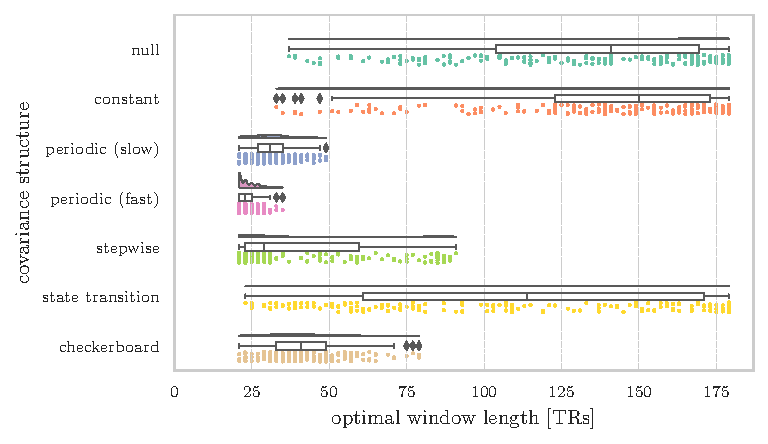
\includegraphics[width=\textwidth]{fig/sim/d2/N0400_T0200/no_noise/SW_cross_validated_optimal_window_lengths}
  \caption{
    Simulations benchmark optimal cross-validated window lengths learned from bivariate ($D = 2$) noiseless data for $N = 400$.
    Each dot represents one of $T = 200$ trials.
    Faster changing covariance structures result in shorter learned window lengths.
  }\label{fig:sim-optimal-window-lengths}
\end{figure}


Similarly, we can look at the learned kernel lengthscales $l$ from the trained \gls{wp} model, as shown in \cref{fig:sim-learned-kernel-lengthscales}.
These are consistent with the \gls{sw-cv} approach.
The more static the covariance structure, the larger the learned kernel lengthscales will be.
The faster the covariance structure changes over time, the smaller the learned kernel lengthscales becomes.
Interestingly, the constant case yields larger kernel lengthscales.
We attribute this mostly to the fact that the prior of the \gls{wp} assumes uncorrelated time series.
Furthermore, the large values learned for the state transition covariance structure indicate that the models were not able to learn this structure.
%
From this we infer that these two model parameters ($l$ and $\hat{w}$) may capture similar aspects of the covariance structure.


\begin{figure}[t]
  \centering
  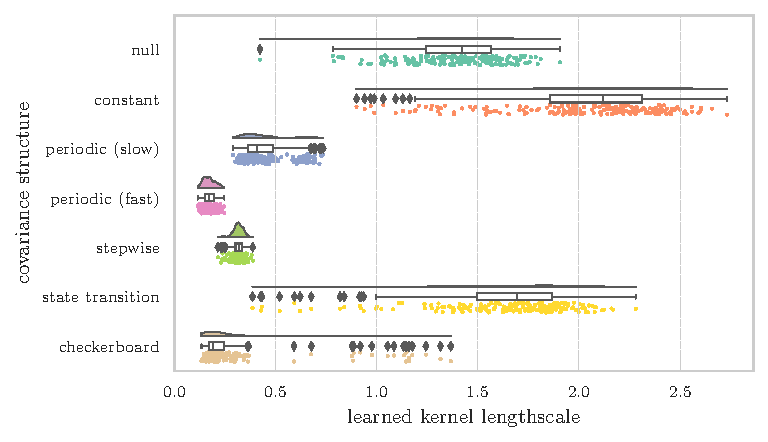
\includegraphics[width=\textwidth]{fig/sim/d2/N0400_T0200/no_noise/SVWP_kernel_lengthscales}
  \caption{
    Simulations benchmark SVWP kernel lengthscales $l$ learned from bivariate ($D = 2$) noiseless data for $N = 400$.
    Each dot represents one of $T = 200$ trials.
    Faster changing covariance structures result in shorter learned kernel lengthscales.
  }\label{fig:sim-learned-kernel-lengthscales}
\end{figure}


One key difference between the optimal window lengths and learned kernel lengthscales is that the latter are more distinct.
For example, given the lengthscales it is possible to perfectly distinguish between the slow and fast periodic covariance structures.
This is not the case for the window lengths, where there is still an overlap between these.

Another important observation is that even for the null and constant cases, our current implementation of \gls{sw-cv} still finds short optimal window lengths in some (rare) cases.
The same can be said for the \gls{wp} kernel lengthscales, although to a lesser degree.
In \cref{subsec:higher-dimensions} we touched upon running our models in pairwise fashion, which would increase the number of window length searches from 1 to $\frac{D (D - 1)}{2}$.
As such we would expect some edges to report false positives.
Perhaps the temporal character of some edges is truly different from others (requiring a different window length or different kernel lengthscale), but this warrants caution.

%%
\subsubsection{Bivariate case}
%%

We start with a qualitative visual inspection of bivariate \gls{tvfc} estimates.
Single trial examples for each method on the simulated data with $N = 400$ for all covariance structures are shown in \cref{fig:sim-results-tvfc-estimates-example}.
Both noiseless (\cref{fig:sim-results-bivariate-no-noise-all-covariance-structures-tvfc-predictions}) and the hybrid case with added \gls{hcp} \gls{rs-fmri} noise with an \gls{snr} of 2 (\cref{fig:sim-results-bivariate-HCP-noise-all-covariance-structures-tvfc-predictions}) are shown.
Results for other values of $N$ and noise configurations can be found in \cref{ch:appendix-d2-impact-of-noise}.


\begin{figure}[t]
  \centering
  \subcaptionbox{Without noise\label{fig:sim-results-bivariate-no-noise-all-covariance-structures-tvfc-predictions}}{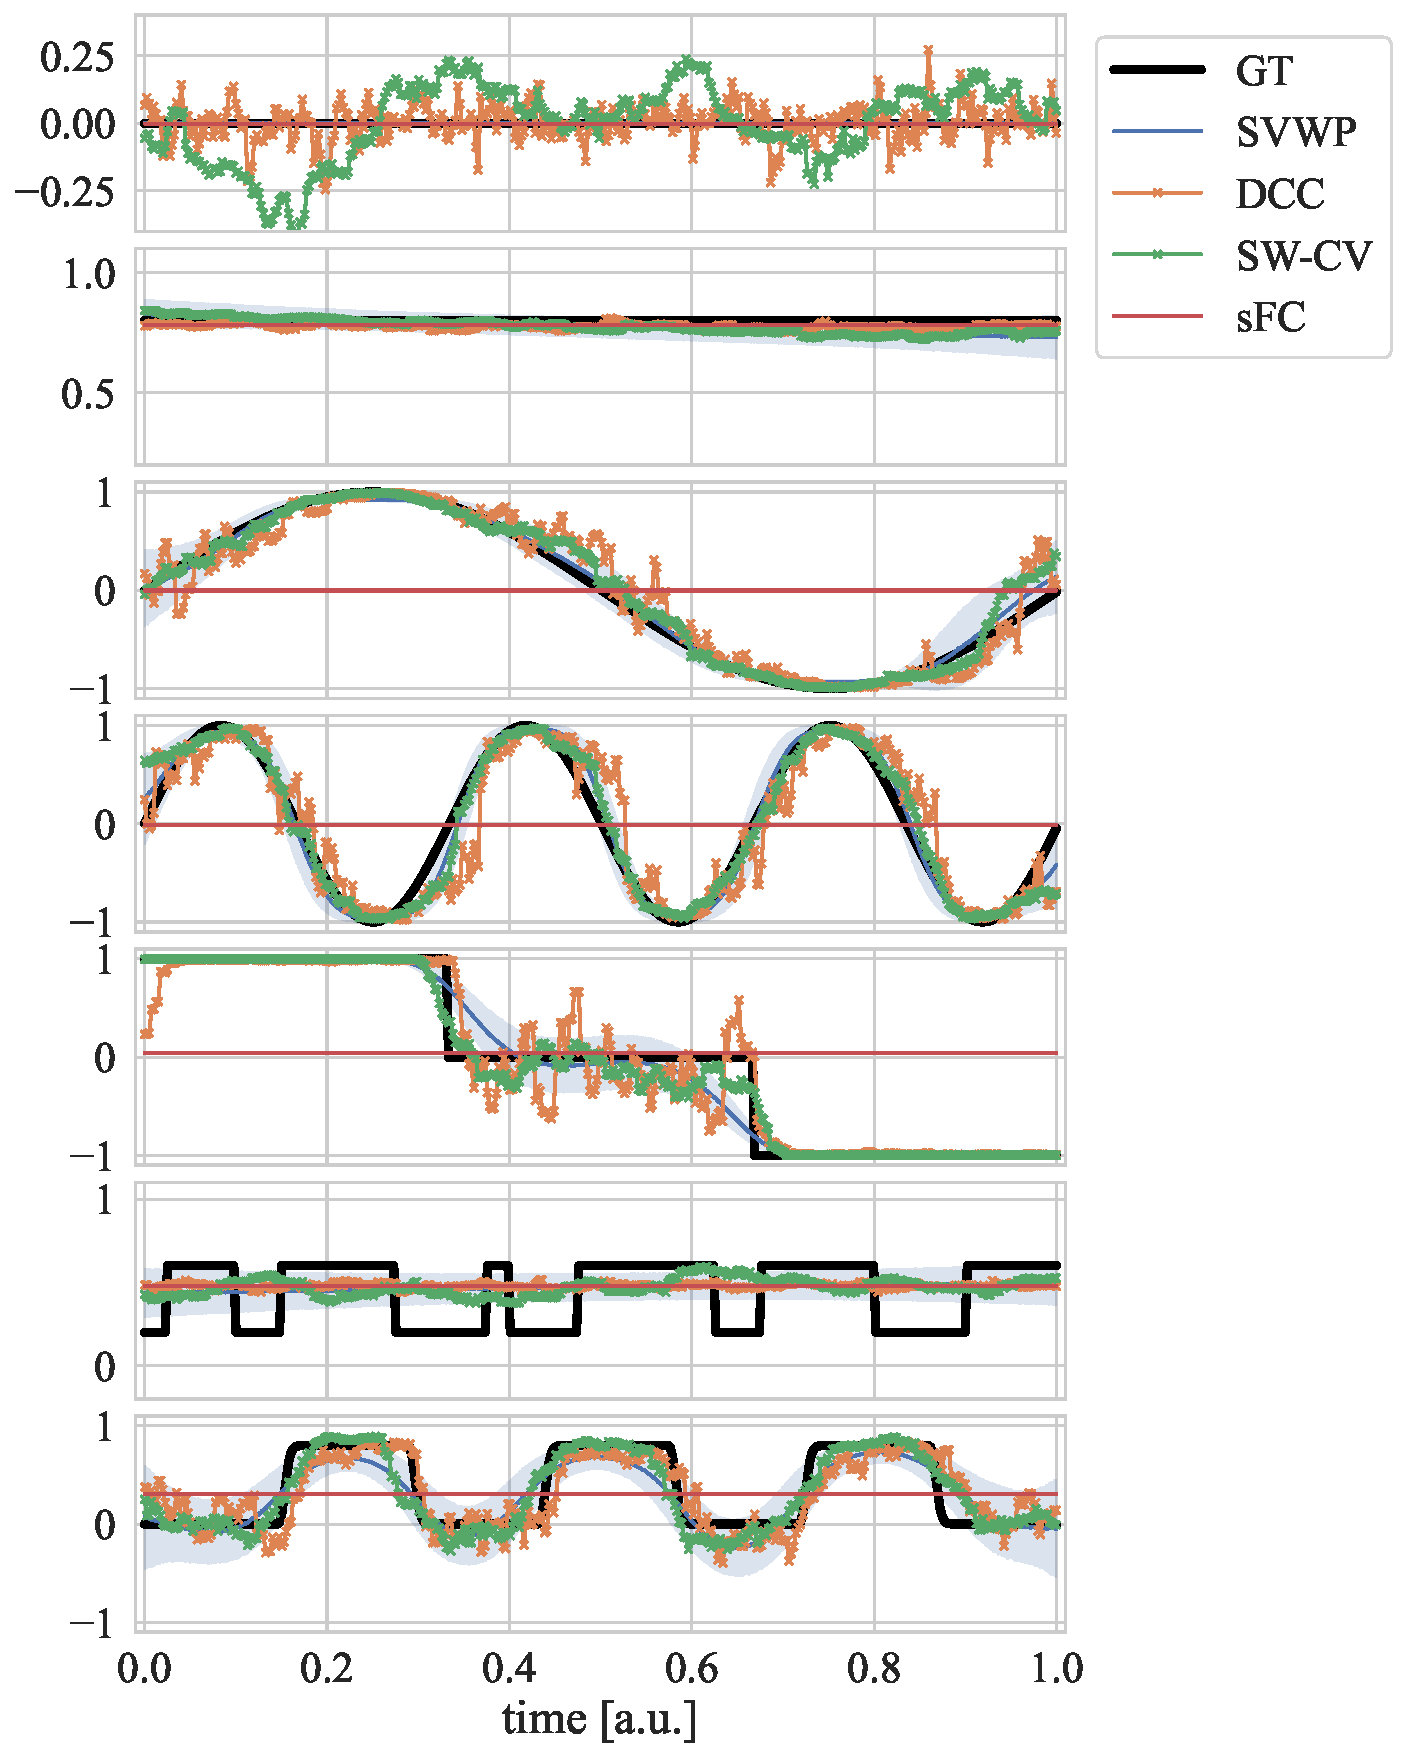
\includegraphics[width=0.48\textwidth]{fig/sim/d2/N0400_T0200/no_noise/all_covs_types_correlations}}
  \subcaptionbox{With rs-fMRI noise (hybrid)\label{fig:sim-results-bivariate-HCP-noise-all-covariance-structures-tvfc-predictions}}{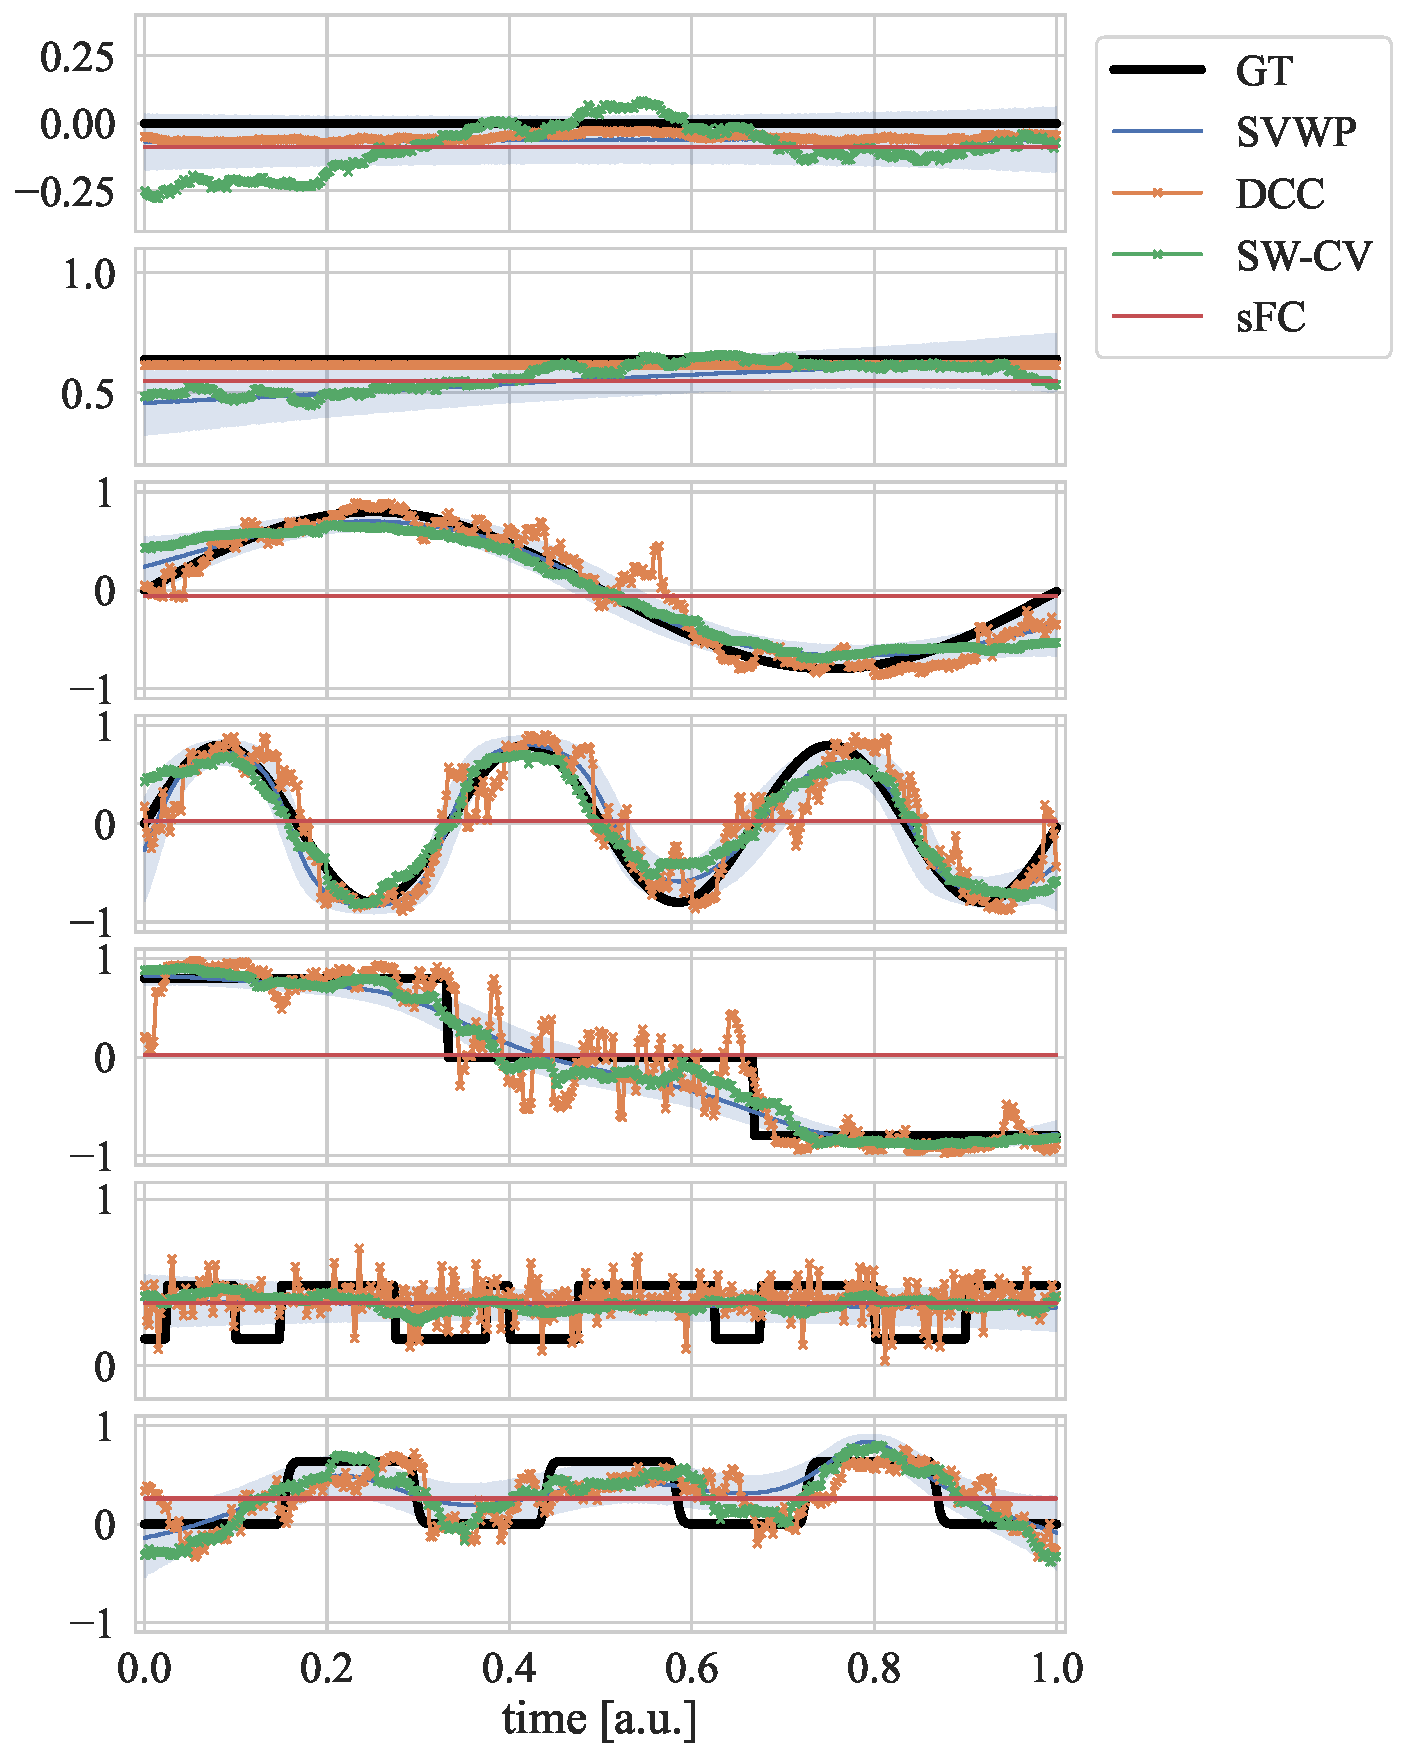
\includegraphics[width=0.48\textwidth]{fig/sim/d2/N0400_T0200/HCP_noise_snr_2/all_covs_types_correlations}}
  \caption{
    Simulations benchmark single trial TVFC estimates for all covariance structures, for bivariate data ($D = 2$) for $N = 400$.
    Ground truth (GT) is included for reference.
    Estimation methods have distinct failure modes.
  }\label{fig:sim-results-tvfc-estimates-example}
\end{figure}


Failure modes of the different \gls{tvfc} estimation methods are clearly visible.

For the two static covariance structures (null and constant), even the cross-validated \gls{sw} method detects spurious time-varying structure.
This \gls{sw} failure mode has been long known in the field~\parencite{Lindquist2014, Hindriks2016}.
The \gls{dcc} and \gls{svwp} models remain close to the ground truth.

For the two periodic covariance structures, the \gls{sfc} estimate is not sensitive to this structure, unlike for the null and constant covariance structure data.
\gls{sw-cv} performs well and picks the correct window length in both cases.
The \gls{mgarch} model captures the structure as well, although spurious sudden large jumps are seen.
We see that the \gls{svwp} can model smooth changes in covariance structure well (indeed, this is perhaps where it excels).
From visual inspection it seems to return the best fit.
It is worth pointing out as well that the \gls{sw-cv} estimates at all time steps fall within the uncertainty bounds of the \gls{svwp} estimates.

For the stepwise data, we can see that the \gls{svwp} estimates are too smooth and perform poorly during sudden changes in covariance structure.
This is an expected failure mode, as this model expects slowly changing covariance.
Moreover, the `static' part of the time series requires a longer lengthscales, whereas the sudden jumps would require a shorter lengthscales.
The \gls{sw-cv} estimates suffer from a similar problem, where it is not clear what window length would be optimal here.
The \gls{dcc} method deals well with the change points but shows a lot of jumps in the middle of the time series.
As they are autoregressive models, they do not work well for the beginning of the time series either.
This could be mitigated, however, by removing the first several volumes from the analysis, which is common practice in \gls{fmri} studies (usually no more than six).
These first volumes are often considered unreliable because the participant and scanner are `settling in' during these.
Crucially, these plots show that estimates are vastly different in nature, and without knowing our eventual use case it is hard to say which estimates are superior here.

All methods fail to pick up the state transition covariance structure, although in different ways.
The \gls{svwp} predicts like it is static (with a large uncertainty bound), and \gls{dcc} and \gls{sw} estimates jump around a little, sometimes seemingly capturing some of the structure.
Interestingly, these estimates look like the ones made for the static covariance cases.
So, if we would have not known any ground truth, it would have been unclear if the underlying process was static or showed state transitions as simulated here.
The fact that none of the methods can pick up on this structure also raises concern about whether we need completely different approaches if such underlying structure is to be expected in real data.
How subtle do we expect changes in \gls{tvfc} with shifting cognitive state?
How many of such changes do we expect per minute?
We will return to this issue in \cref{subsec:sudden-changes}.

Finally, for the checkerboard data, all time-varying methods pick up generally on the covariance structure.
Method characters are different, however, with the \gls{svwp} estimates again being overly smooth and the other methods estimating many discontinuities.
There are several trials where the \gls{svwp} fails to learn the structure for lower values of $N$.


\begin{figure}[ht]
  \centering
  \subcaptionbox{Bivariate case ($D = 2$)\label{fig:sim-results-d2-HCP-noise-all-correlation-RMSE}}{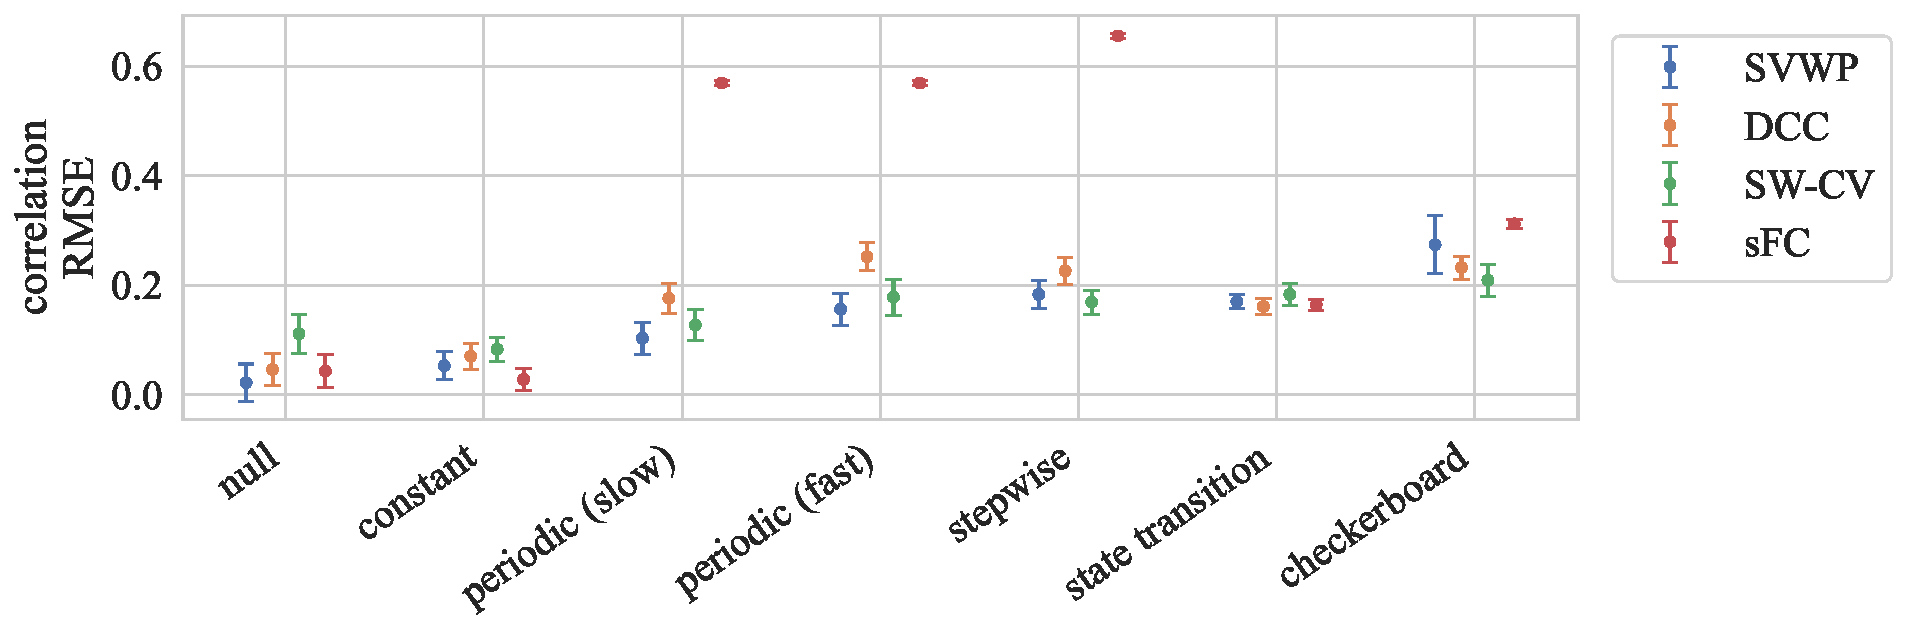
\includegraphics[width=0.84\textwidth]{fig/sim/d2/N0400_T0200/HCP_noise_snr_2/correlation_RMSE}}
  \subcaptionbox{Trivariate dense case ($D = 3$)\label{fig:sim-results-d3d-HCP-noise-all-correlation-matrix-RMSE}}{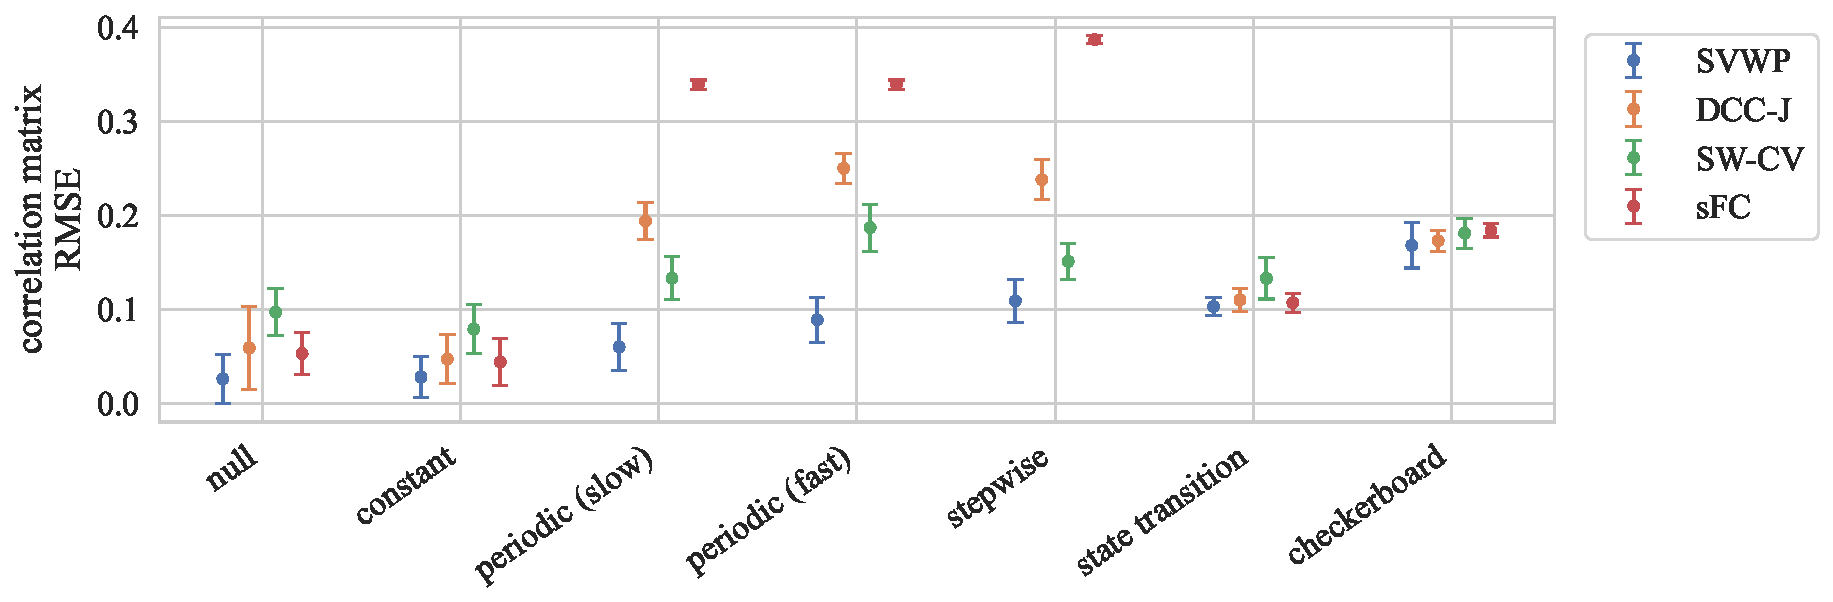
\includegraphics[width=0.84\textwidth]{fig/sim/d3d/N0200_T0200/HCP_noise_snr_2/correlation_matrix_RMSE}}
  \subcaptionbox{Trivariate sparse case ($D = 3$)\label{fig:sim-results-d3s-HCP-noise-all-correlation-matrix-RMSE}}{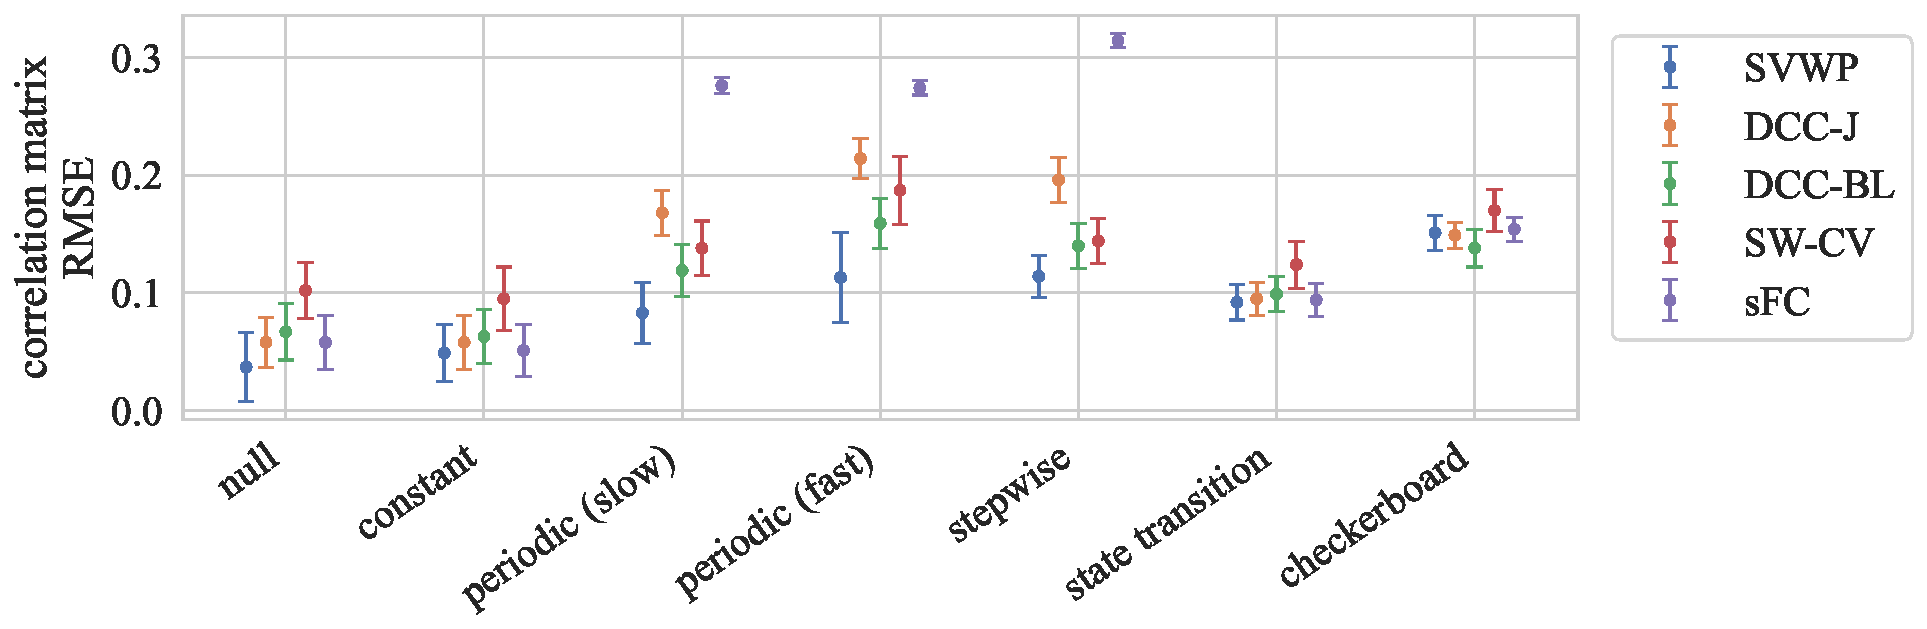
\includegraphics[width=0.84\textwidth]{fig/sim/d3s/N0200_T0200/HCP_noise_snr_2/correlation_matrix_RMSE}}
  \caption{
    Simulations benchmark RMSE between model TVFC estimates and ground truth on all bivariate and trivariate covariance structures with added rs-fMRI noise (SNR of 2) for $N = 400$.
    Means and standard deviations are shown across $T = 200$ trials.
  }\label{fig:sim-results-HCP-noise-all}
\end{figure}


Although the visual inspection of this single trial gives us intuition for model performance and failure modes, to compare methods robustly we need to \emph{quantify} model performance.
The computed \gls{rmse} between estimated and ground truth correlation terms (i.e.~the off-diagonal term) is shown in \cref{fig:sim-results-d2-HCP-noise-all-correlation-RMSE}.
The results are shown for the hybrid case, as a noisier setup is considered more realistic.
%
These quantitative results generally confirm our intuition from the visual inspection.
The \gls{svwp} and \gls{dcc} models perform like a single window approach for the null and constant cases, with the \gls{sw-cv} performing slightly worse.
The \gls{svwp} is better at modeling the smooth periodic covariance structures, whereas the \gls{dcc} model picks up relatively better on the sudden changes of the stepwise covariance structure.
The \gls{sw-cv} performs well overall on the dynamic covariance structures.
The \gls{sfc} estimate, as expected, performs well on static covariance structures, and fails on the time-varying structure.
Interestingly, the \gls{wp} even \emph{outperforms} \gls{sfc} on null covariance, which is likely due to its prior (mean function) expecting zero correlation.
%
However, none of the methods can significantly outperform the \gls{sfc} estimate on the state transition covariance structure.
This result can be considered a quantitative confirmation of our hypothesis from looking at the estimates.
This structure may be too hard to learn by the methods considered.
This point was made by \textcite{Lindquist2014} too, who claimed that \gls{dcc} cannot model abrupt changes (change points) well.
Results for $N = 120$, $N = 200$, and $N = 1200$ show similar relative performance (see \cref{appendix:sim-more-quantitative-results}).
%
Model estimates may look different despite having similar reconstruction errors, as is the case for the stepwise covariance structure, for example.
This highlights the limit of using such a performance metric alone.
%
Lastly, based on these results we posit that a method's outperformance of the \gls{sfc} can be considered an indication of how time-varying the covariance structure is.
If a dynamic method's performance is similar to that of \gls{sfc}, either there is no or little dynamic structure present, or the method has failed to pick up on it (e.g.~state transition).

%%
\subsubsection{Trivariate cases}
%%

Recall that for the trivariate ($D = 3$) case we train \gls{dcc} both in a pairwise and joint manner.
Some illustrative \gls{tvfc} estimates are shown in \cref{ch:appendix-d3-tvfc-estimates}.
We make similar observations as for the bivariate case.
For the null case (\cref{fig:results-d3-no-noise-null-covariance}) we see that the \gls{sw-cv} estimates still return time-varying structure.
Interestingly, the pairwise \gls{dcc} here performs worse than the jointly trained one.
This may be due to this \gls{dcc} still returning spurious structure when given just two time series (as we have seen in the bivariate case).
For the dense trivariate case (\cref{fig:results-d3s-no-noise-periodic-3-covariance}) we see \gls{tvfc} estimates similar to the ones for the bivariate case.
However, the sparse case (\cref{fig:results-d3s-no-noise-stepwise-covariance}) reveals that it may be a good idea to train \gls{dcc} in a pairwise manner.
The jointly trained \gls{dcc} model performs much worse here.

Quantitative results for the dense and sparse trivariate cases with added \gls{hcp} \gls{rs-fmri} noise are shown in \cref{fig:sim-results-d3d-HCP-noise-all-correlation-matrix-RMSE} and \cref{fig:sim-results-d3s-HCP-noise-all-correlation-matrix-RMSE}.
We generally see the same trends in these results as for the bivariate case.
The \gls{svwp} does relatively well on the sparse covariance structures, and the jointly trained \gls{dcc} does relatively poorly here.

%%
\subsubsection{Toward higher dimensions}
%%

Real applications would typically have more than $D = 3$ nodes (e.g. 15, 6, 9, and 3 for the subsequent respective studies in this thesis).
The sparse implementation can be scaled to any number of dimensions.
Running this on higher dimensions maintains the same trends as we saw for the bivariate and trivariate cases.
However, more complicated covariance structures in higher dimensions are left for future work.

%%
\subsubsection{Impact of noise analysis}\label{subsec:impact-of-noise-analysis}
%%

To understand the impact of noise on our results, the estimates for various noise levels are shown in \cref{ch:appendix-d2-impact-of-noise,ch:appendix-d3d-impact-of-noise}.
All methods gradually perform worse with lower \glspl{snr}.
We see most methods breaking down with the \gls{snr} of 1.
However, some methods break down before others.

%%
\subsubsection{Imputation benchmark}
%%

The imputation benchmark (\cref{subsec:imputation-benchmark}) is also run on all synthetic covariance structures.
We are mainly interested in comparing the performance on this benchmark to the reconstruction errors discussed before.
%
Let us look at two cardinal cases, both using bivariate, noiseless data.
For the null covariance case (\cref{fig:sim-imputation-study-d2-null}), we find all methods to perform similarly well on the imputation benchmark.
This was to be expected.
All models can model this appropriately, as witnessed in both the visual inspection and the quantified results.
\gls{sw-cv} performs slightly worse than the other methods, which again was to be expected as it also performed slightly worse on the other performance metrics.
However, for a non-static covariance structure such as the slowly oscillating periodic one, we find the \gls{sfc} estimates to perform much worse on the imputation benchmark than the other methods (see \cref{fig:sim-imputation-study-d2-periodic-1}).
We find the \gls{svwp} to perform best on this benchmark.
Thus, we obtained results \emph{without} using a ground truth, that correspond well to the performance metrics computed \emph{with} knowledge of a ground truth.
This is exciting, as this imputation benchmark can be run on any (real) data set.


\begin{figure}[t]
  \centering
  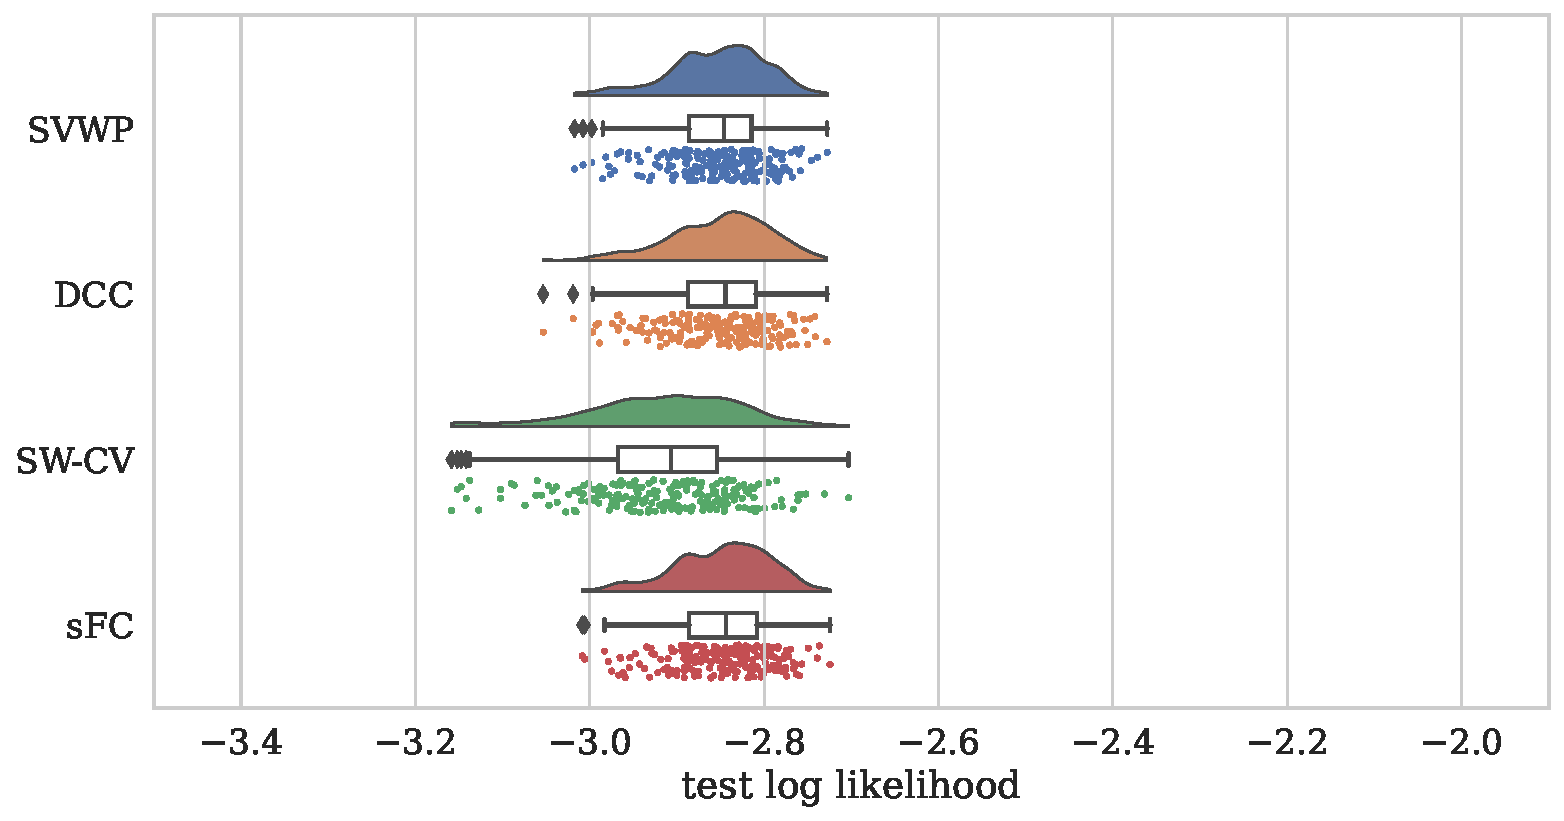
\includegraphics[width=\textwidth]{fig/sim/d2/N0400_T0200/imputation_study/LEOO_no_noise_test_log_likelihoods_raincloud_null}
  \caption{
    Simulations imputation benchmark - null covariance.
    Test log likelihoods for bivariate ($D = 2$) noiseless data for $N = 400$.
    Each dot represents one of $T = 200$ trials.
  }\label{fig:sim-imputation-study-d2-null}
\end{figure}


\begin{figure}[t]
  \centering
  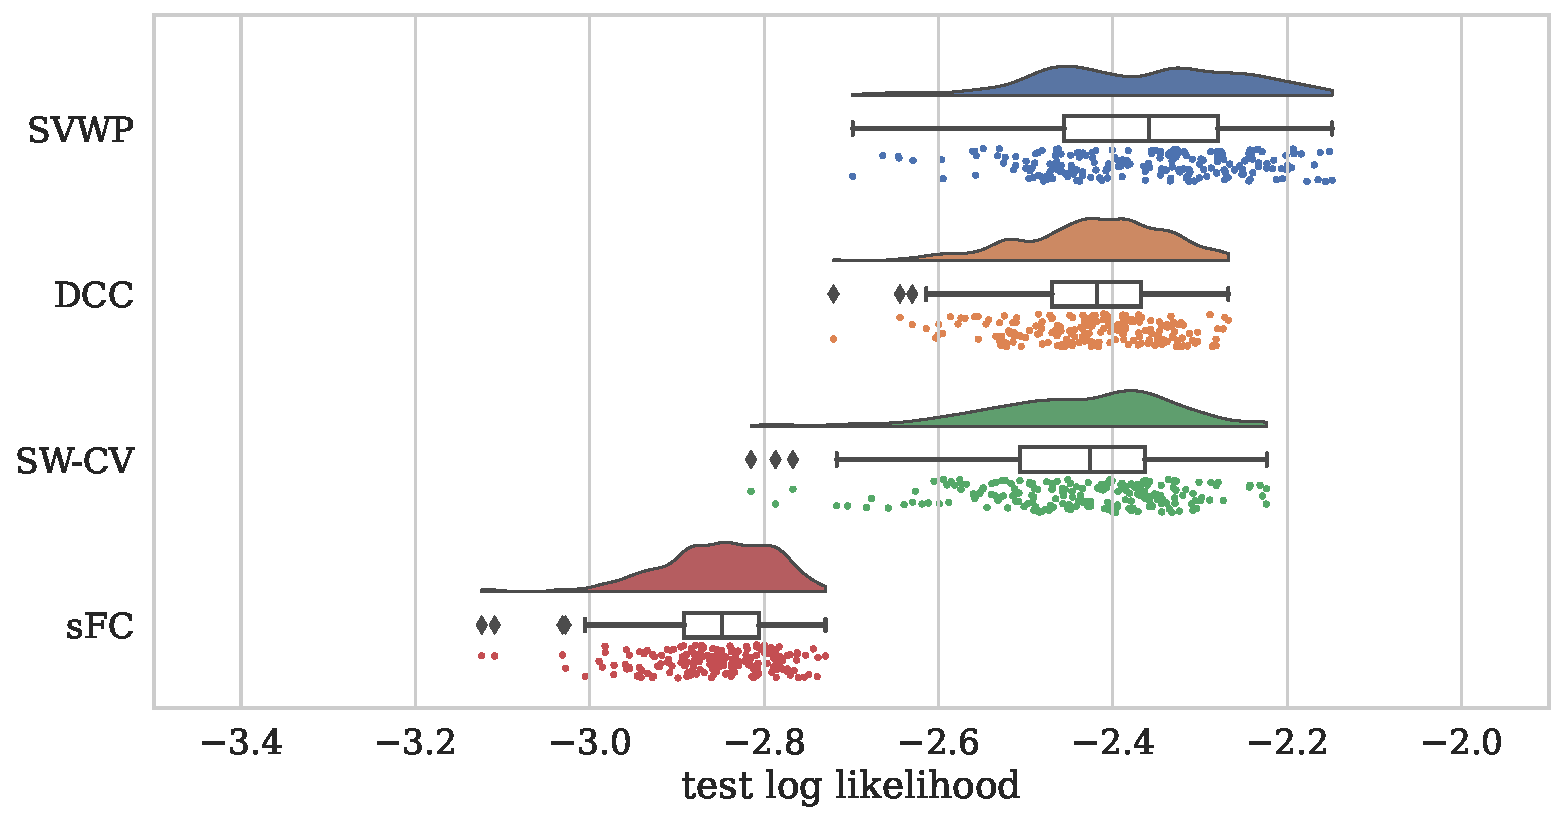
\includegraphics[width=\textwidth]{fig/sim/d2/N0400_T0200/imputation_study/LEOO_no_noise_test_log_likelihoods_raincloud_periodic_1}
  \caption{
    Simulations imputation benchmark - periodic (slow) covariance.
    Test log likelihoods for bivariate ($D = 2$) noiseless data for $N = 400$.
    Each dot represents one of $T = 200$ trials.
  }\label{fig:sim-imputation-study-d2-periodic-1}
\end{figure}


%%
\clearpage
\subsection{Resting-state fMRI}\label{subsec:hcp-results}
%%

Before diving into any quantitative results, we should again visually inspect the estimated \gls{tvfc} from different methods.
This time we study a real \gls{fmri} data set.
Estimates for several edges of a single scan of a single subject from the \gls{hcp} data set ($D = 15$) are shown in \cref{fig:hcp-model-estimates-example}.


\begin{figure}[ht]
  \centering
  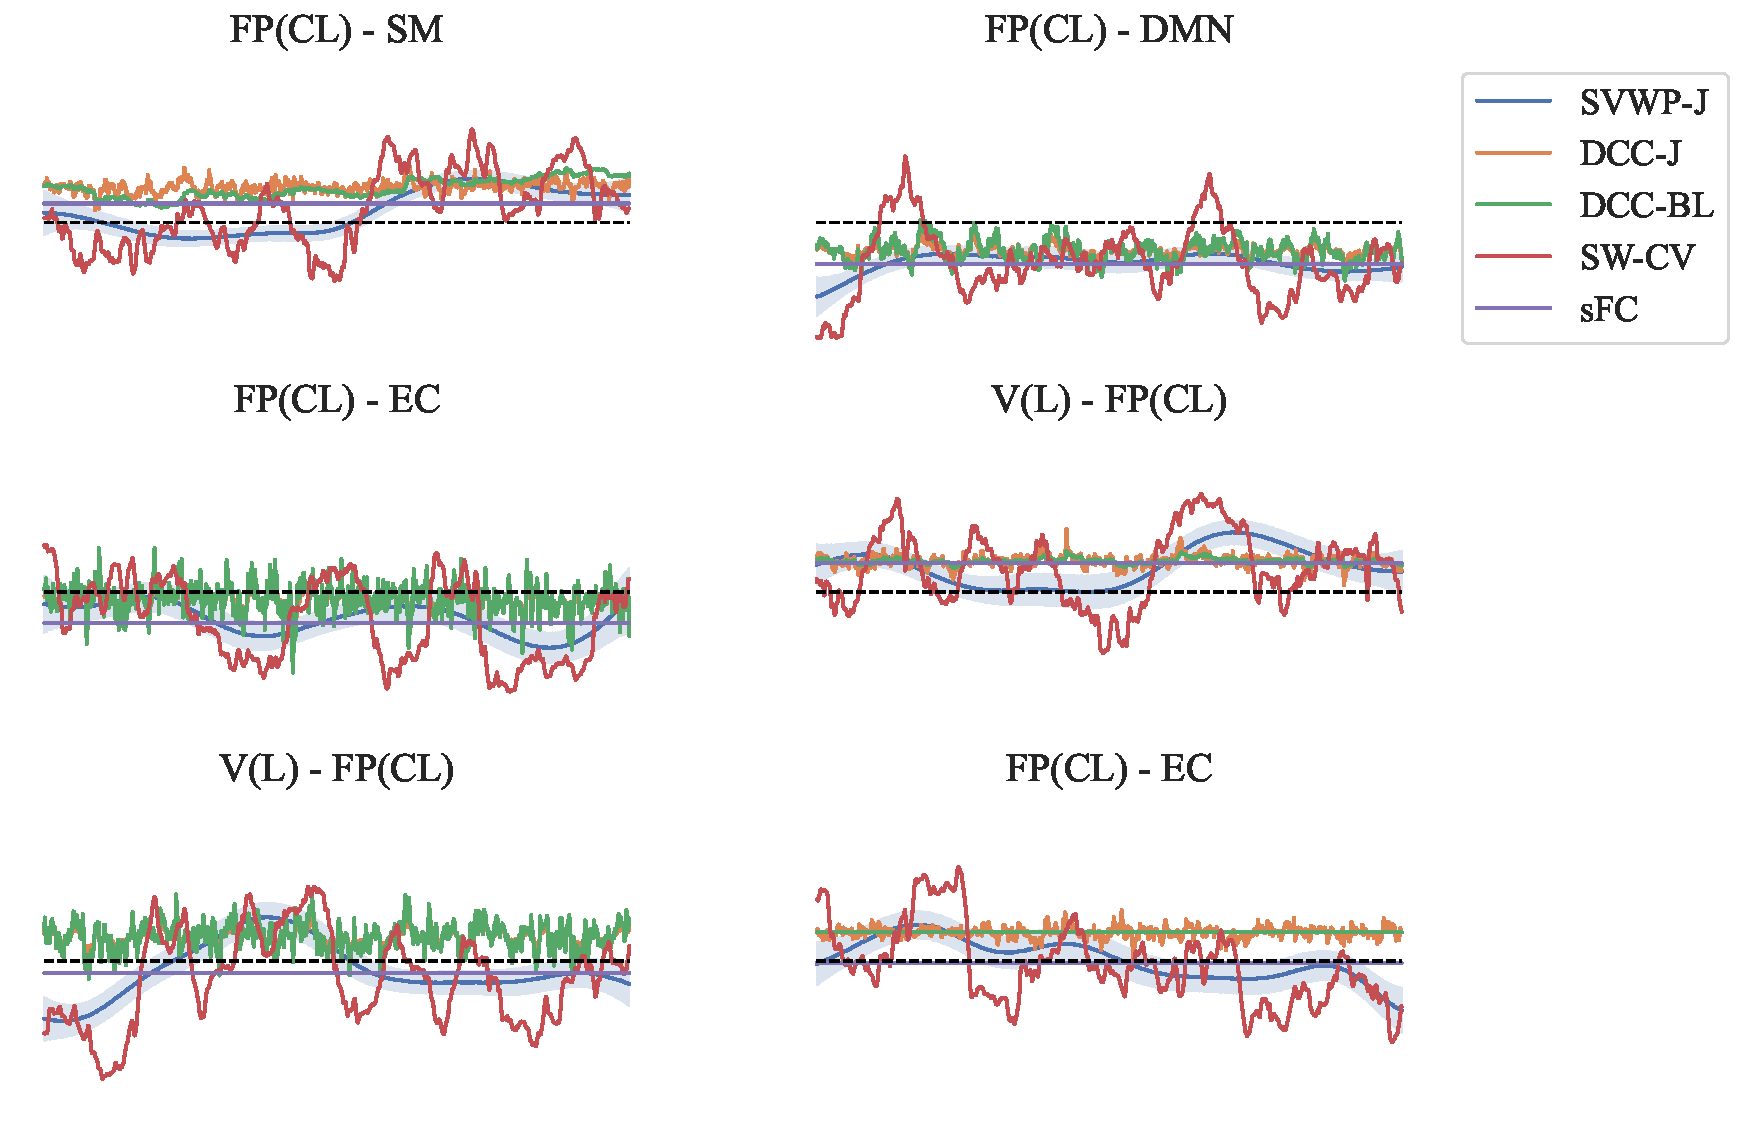
\includegraphics[width=\textwidth]{fig/hcp/d15/TVFC_predictions/scan_0/all/100206/correlation_estimates_random_edges}
  \caption{
    HCP benchmark TVFC estimates for random selection of edges (from $D = 15$ time series) for a single scan of a single HCP subject.
    The y-axis scales from~-1~to~1; the black dashed line indicates zero correlation.
    Method estimates vary radically.
}\label{fig:hcp-model-estimates-example}
\end{figure}


Several observations can be made from visual inspection.
%
First, there is a large variety in general correlation (connectivity strength) between the edges.
Albeit with fluctuations, some edges are consistently strongly correlated, whereas others are generally uncorrelated.
Some edges show dynamics, whereas others appear more static.
This was to be expected, as brain region interactions should be distinct from one another.
%
Secondly, perhaps worryingly, estimates vary radically among the methods considered.
The mean of \gls{tvfc} estimates across time for both the \gls{svwp} and \gls{sw} methods is consistent with the \gls{sfc} estimate, in contrast to the \gls{dcc} estimates.
We also see major differences between \gls{tvfc} estimates in terms of how fast \gls{tvfc} changes.
The \gls{sw} method estimates constantly and rapidly changing \gls{tvfc}, with large variance across time.
The \gls{svwp} method estimates time-varying but transiently changing \gls{tvfc}.
The \gls{dcc} method estimates rapidly changing \gls{tvfc}, but constricted to a small range (i.e.~low variance).
%
Lastly, we observe that the \gls{svwp} estimates look like a smooth version of the \gls{sw-cv} estimates.
This could mean that either the \gls{svwp} model cannot pick up on the fast-changing nature of \gls{tvfc}, or that the \gls{sw-cv} method picks up on spurious fluctuations (yet still captures the general trends).
Training \gls{dcc} in a joint or pairwise manner does not seem to make a significant difference here.
%
These insights have been qualitatively verified by inspecting other scans.


\begin{figure}[t]
  \centering
  \subcaptionbox{SVWP-J\label{fig:HCP-model-estimates-summary-measures-mean-SVWP}}{\includegraphics[width=0.30\textwidth]{fig/hcp/d15/TVFC_predictions_summaries/scan_0/all/correlation_TVFC_mean_SVWP_joint}}
  \subcaptionbox{DCC-J\label{fig:HCP-model-estimates-summary-measures-mean-DCC}}{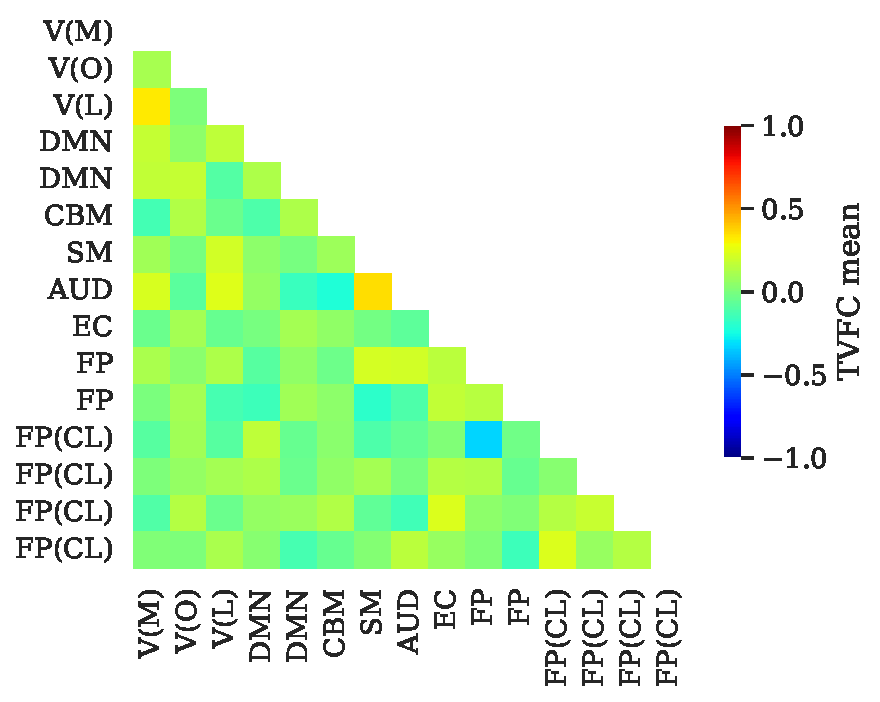
\includegraphics[width=0.30\textwidth]{fig/hcp/d15/TVFC_predictions_summaries/scan_0/all/correlation_TVFC_mean_DCC_joint}}
  \subcaptionbox{SW-CV\label{fig:HCP-model-estimates-summary-measures-mean-SW}}{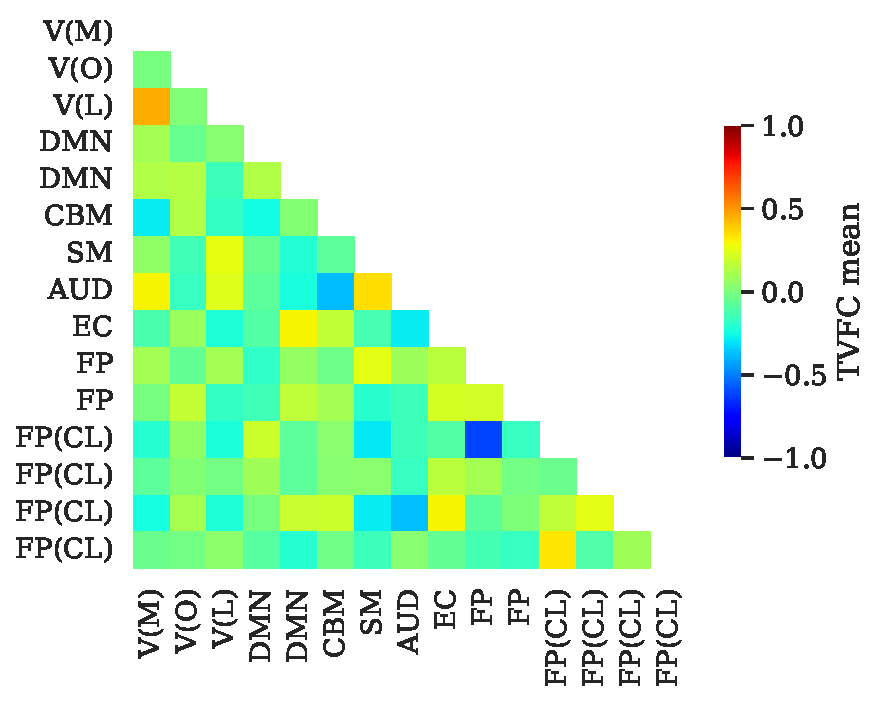
\includegraphics[width=0.30\textwidth]{fig/hcp/d15/TVFC_predictions_summaries/scan_0/all/correlation_TVFC_mean_SW_cross_validated}}
  \subcaptionbox{SVWP-J\label{fig:HCP-model-estimates-summary-measures-var-SVWP}}{\includegraphics[width=0.30\textwidth]{fig/hcp/d15/TVFC_predictions_summaries/scan_0/all/correlation_TVFC_variance_SVWP_joint}}
  \subcaptionbox{DCC-J\label{fig:HCP-model-estimates-summary-measures-var-DCC}}{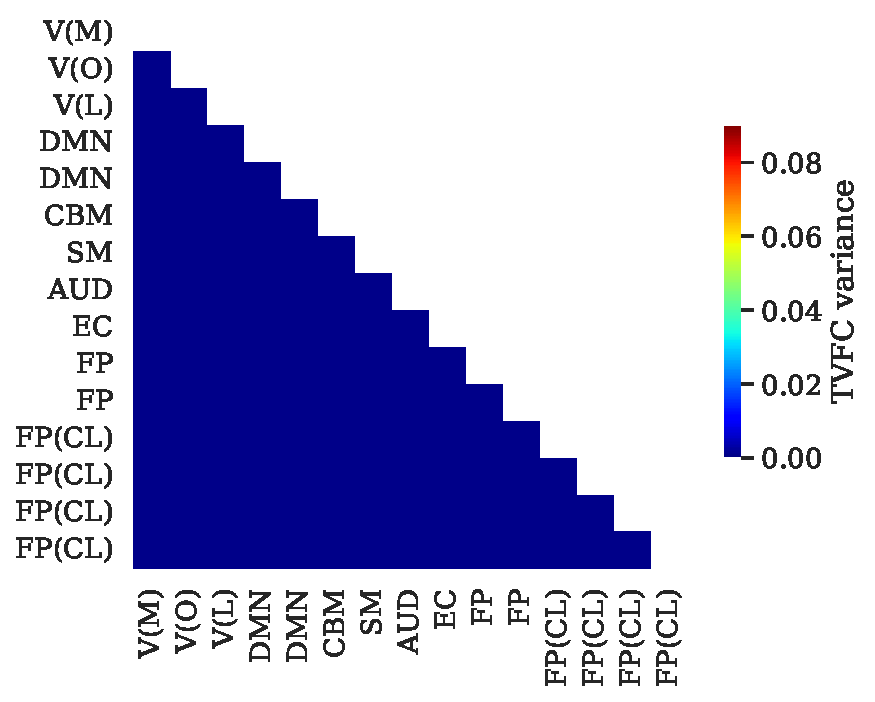
\includegraphics[width=0.30\textwidth]{fig/hcp/d15/TVFC_predictions_summaries/scan_0/all/correlation_TVFC_variance_DCC_joint}}
  \subcaptionbox{SW-CV\label{fig:HCP-model-estimates-summary-measures-var-SW}}{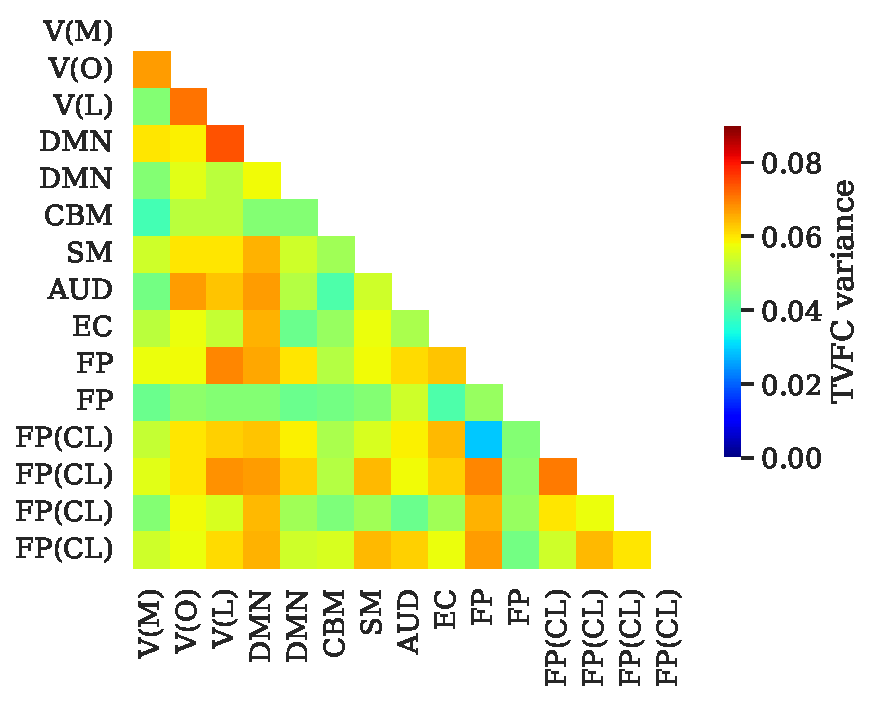
\includegraphics[width=0.30\textwidth]{fig/hcp/d15/TVFC_predictions_summaries/scan_0/all/correlation_TVFC_variance_SW_cross_validated}}
  \subcaptionbox{SVWP-J\label{fig:HCP-model-estimates-summary-measures-roc-SVWP}}{\includegraphics[width=0.30\textwidth]{fig/hcp/d15/TVFC_predictions_summaries/scan_0/all/correlation_TVFC_rate_of_change_SVWP_joint}}
  \subcaptionbox{DCC-J\label{fig:HCP-model-estimates-summary-measures-roc-DCC}}{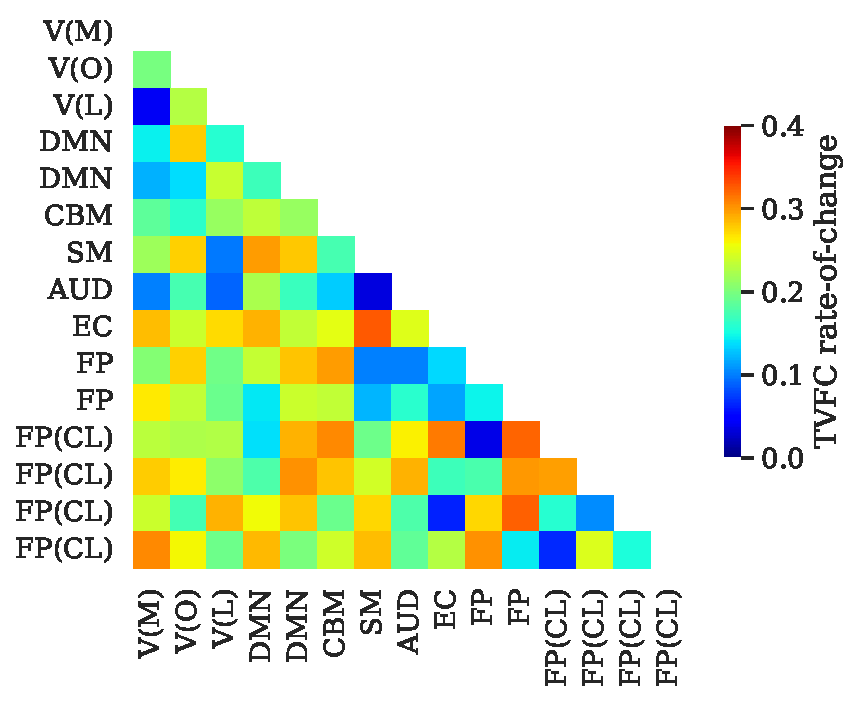
\includegraphics[width=0.30\textwidth]{fig/hcp/d15/TVFC_predictions_summaries/scan_0/all/correlation_TVFC_rate_of_change_DCC_joint}}
  \subcaptionbox{SW-CV\label{fig:HCP-model-estimates-summary-measures-roc-SW}}{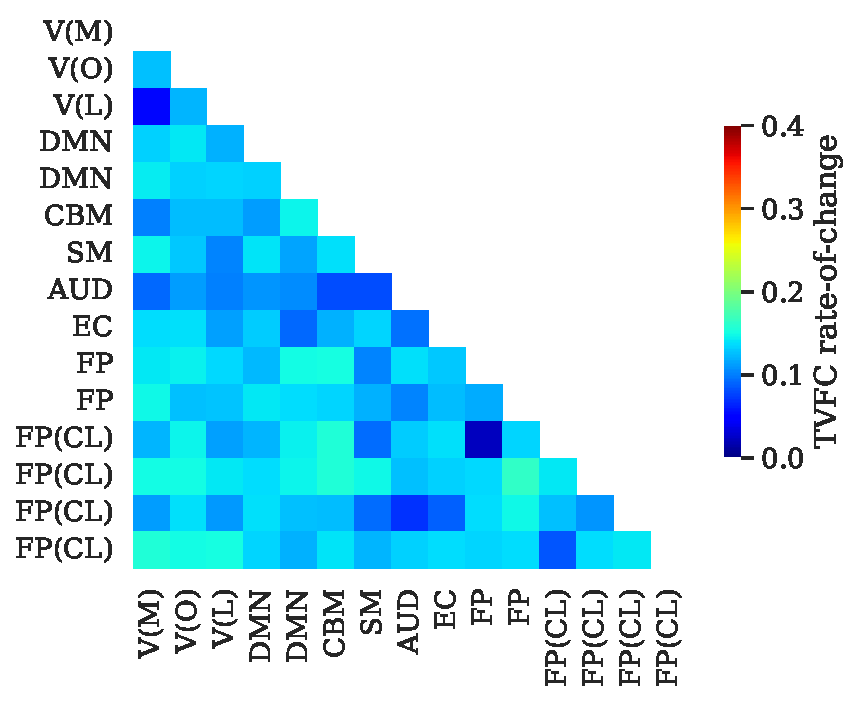
\includegraphics[width=0.30\textwidth]{fig/hcp/d15/TVFC_predictions_summaries/scan_0/all/correlation_TVFC_rate_of_change_SW_cross_validated}}
  \caption{
    HCP benchmark edgewise TVFC summary measures of first scan (1A) averaged over all subjects.
    TVFC mean (top), variance (middle), and rate-of-change (bottom row) are shown.
    For interpretation, ICA components are mapped to FNs.
    Visual (V): medial (M), occipital (O), lateral (L); Default Mode Network (DMN); Cerebellum (CBM); Sensorimotor (SM); Auditory (AUD); Executive Control (EC); Frontoparietal (FP) with Cognition-Language (CL) subset.
  }\label{fig:HCP-model-estimates-summary-measures}
\end{figure}


These distinct differences in dynamics can be captured by three \gls{tvfc} summary measures: mean, variance, and rate-of-change (see \cref{subsec:tvfc-summary-measures}), as shown in \cref{fig:HCP-model-estimates-summary-measures}.
Our broad intuition from the visual inspection holds for these summary measures.
%
The mean estimates across these three methods looks similar, although the \gls{dcc} means are slightly different.
%
For variance, we see small values for \gls{dcc}, large values for \gls{sw-cv}, and the values for \gls{svwp} estimates in between these.
%
For rate-of-change, we see smaller values for both the \gls{svwp} and \gls{sw-cv}, and larger values for \gls{dcc}.
%
From this inspection we may conclude that the combined three summary measures paint a reasonably comprehensive summary of each method's \gls{tvfc} estimates.
The summary measures of the pairwise \gls{dcc} estimates are similar to the joint ones.


\begin{figure}[t]
  \centering
  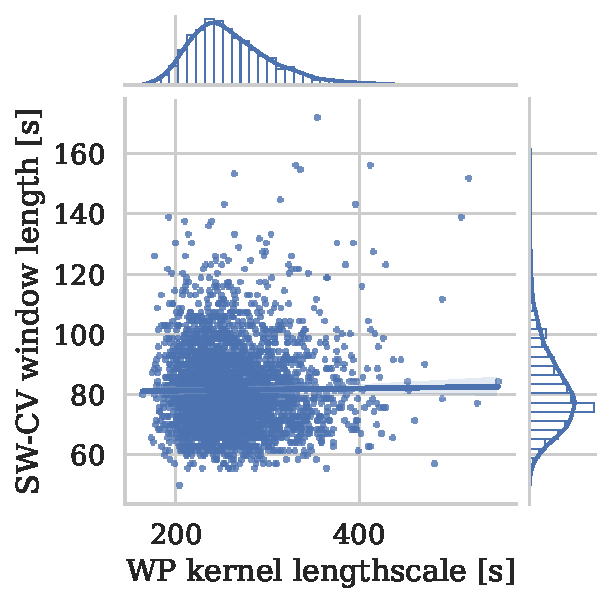
\includegraphics[width=0.45\textwidth]{fig/hcp/d15/lengthscale_optimal_window_length_relations}
  \caption{
    HCP benchmark relationship between learned SVWP kernel lengthscales (scaled to time series length) and SW-CV optimal window length.
    Each dot represents one of four scans (1A, 1B, 2A, 2B) for each subject.
    Full time series are 864 seconds long.
  }\label{fig:sim-relationship-lengthscale-optimal-window-length}
\end{figure}


As we see that the \gls{svwp} and \gls{sw-cv} estimates are distinct in this case, we compare the learned \gls{svwp} kernel lengthscales with the estimated optimal window lengths (similar to \cref{fig:sim-optimal-window-lengths} and \cref{fig:sim-learned-kernel-lengthscales}).
Perhaps surprisingly, despite prior evidence that these two hyperparameters may pick up on similar aspects of the data, we do not find a significant relationship between them here across all scans, as shown in \cref{fig:sim-relationship-lengthscale-optimal-window-length}.
One explanation for this could be that these learned hyperparameters are mostly related to the variance summary measure (where \gls{svwp} and \gls{sw-cv} estimates are quite distinct) rather than the rate-of-change summary measure (where they are more similar).
Alternatively, it may be the case that with the simulations the covariance structures were much more distinct, whereas in this actual data set the dynamics between edges may not differ as much.
These two hyperparameters may still correspond to each other, but these results suggest caution.

%%
\subsubsection{Subject measure prediction benchmark}
%%


\begin{figure}[t]
  \centering
  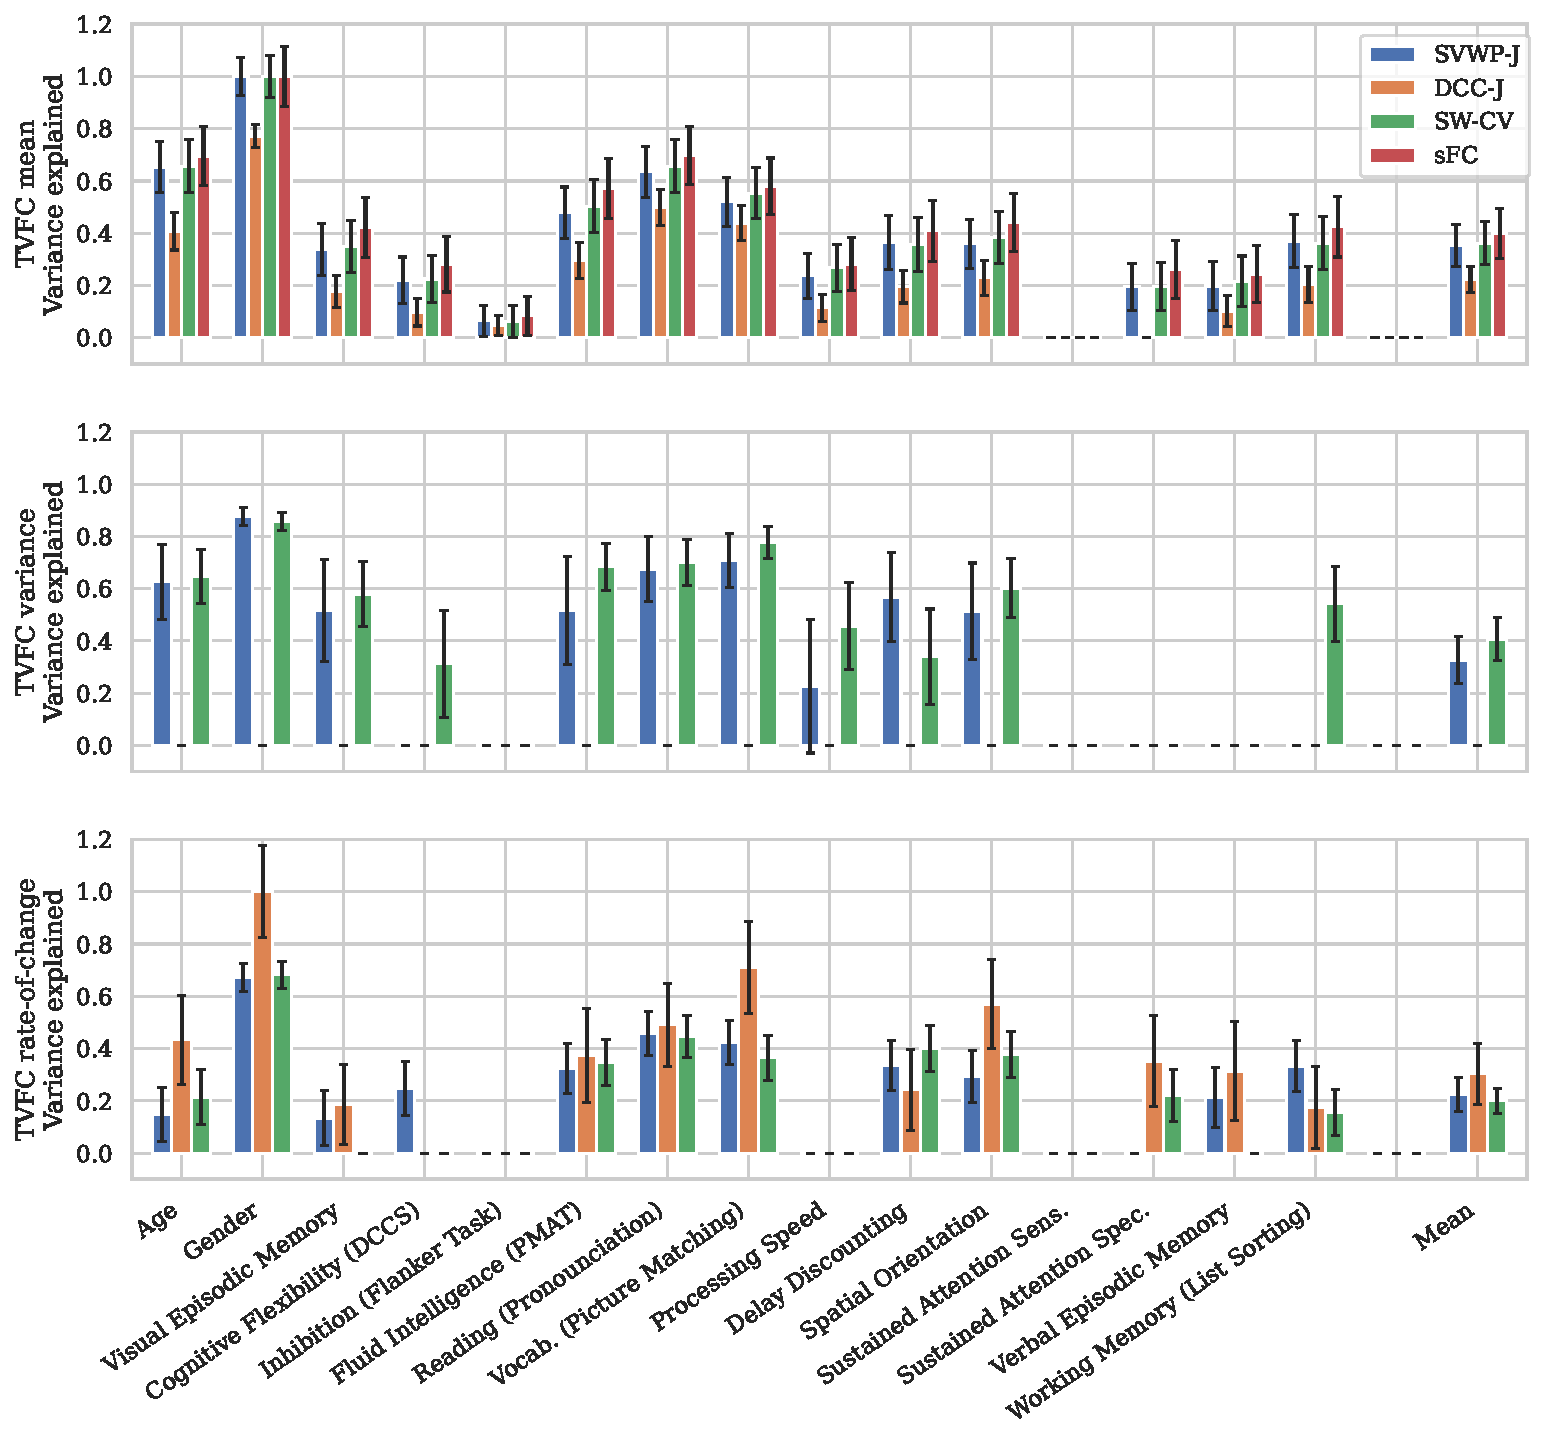
\includegraphics[width=\textwidth]{fig/hcp/d15/subject_measure_prediction/cognitive/morphometricity_all_TVFC_summary_measures}
  \caption{
    HCP benchmark subject cognitive measures prediction morphometricity scores (with standard error).
    Run on TVFC summary measures of mean (top), variance (middle), and rate-of-change (bottom row).
    sFC is added for reference to the TVFC mean plot.
  }\label{fig:hcp-results-subject-measures-prediction}
\end{figure}


Morphometricity (variance explained) scores are shown in \cref{fig:hcp-results-subject-measures-prediction}.
The pairwise \gls{dcc} scores are almost identical to the joint \gls{dcc}, which is unsurprising as the summary measures are almost identical.
Hence, they are left out here.
%
Since we study the same subject measures as \textcite{Li2019a}, we can compare the \gls{sfc} (as a reference or \emph{null} model; the alternative hypothesis that \gls{fc} is static) and \gls{tvfc} estimate means (top row) directly to theirs.
Scores are generally replicated, for example being close to 1 (for all methods) for Gender.
This provides a healthy sanity check.
%
We also see that none of the \gls{tvfc} estimation methods can outperform the \gls{sfc} method regarding mean \gls{fc} (connectivity strength).
This was expected and highlights that we should only look at \gls{tvfc} methods if we are interested in brain connectivity \emph{dynamics}.
However, a good \gls{tvfc} estimation method should still model mean \gls{tvfc} well (i.e.~get as close to \gls{sfc} performance as possible).

We observe several things from these results.
%
First, for some subject measures none of the variance across all \gls{tvfc} summary measures and estimation methods can be explained (see e.g.~Sustained Attention Sens.).
This could indicate that signatures of these respective tasks are not captured by \gls{fc} in general.
%
Second, we observe strong heterogeneity across methods.
There is no clear-cut conclusion on picking a superior method here.
A method may outperform another on one occasion, but not on another.
However, overall the \gls{svwp} and \gls{sw-cv} methods perform best, whereas \gls{dcc} often fails to explain much variance across these measures.\footnote{As another validation of cross-validating window lengths, we ran the \gls{sw} approach with a window length of both 30 and 60 seconds. The \gls{sw-cv} estimates consistently outperformed both of these, even as this would be an unfair, post-hoc comparison.}
Particularly noteworthy is the complete lack of the \gls{dcc} \gls{tvfc} variance estimates to have any predictive power.
This can be interpreted as it being meaningless (which we will later see to be relevant for the test-retest benchmark).
%
In general, it is also promising here that the time-varying summary measures (variance and rate-of-change) contain information about subject measures as well.
This highlights the value of studying \gls{fc} dynamics instead of merely its properties over the full scan.
%
Another observation can be made about how subject measures are expressed.
In fact, this helps us understand what these summary measures capture.
Subject age, for example, seems to affect \gls{tvfc} mean and variance more so than rate-of-change.
Such insights could lead to (careful) biophysical interpretations as well.
For example, \textcite{Hutchison2015} found that \gls{fc} variability over the length of a scan correlates positively with age.
Based on this finding, we would expect \gls{tvfc} variance to be predictive of age (to some degree).
We do indeed find this for the \gls{wp} and \gls{sw-cv} methods but fail to find this for the \gls{dcc} method.
Such comparisons to literature can be used to assess the validity and general usefulness of a \gls{tvfc} estimation method.
%
Finally, we see that the performance of \gls{svwp} and \gls{sw-cv} estimates are generally coordinated (performing well and failing in similar contexts).
This aligns with our prior intuition that these methods may capture similar aspects of the data.


\begin{figure}[t]
  \centering
  \subcaptionbox{SVWP-J\label{fig:test-retest-mean-SVWP-ICCs}}{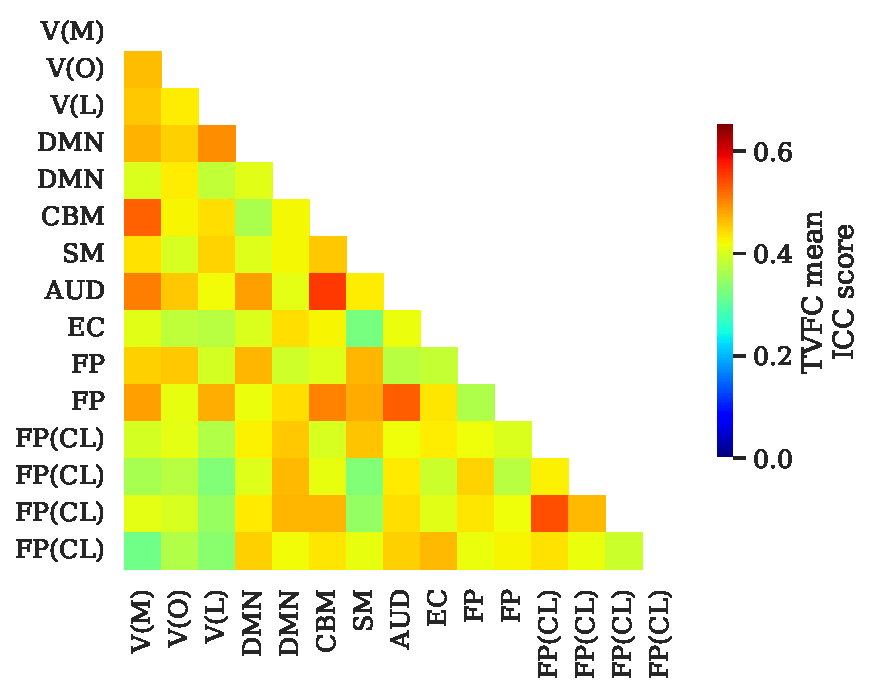
\includegraphics[width=0.28\textwidth]{fig/hcp/d15/test_retest/ICCs/correlation_mean_ICCs_SVWP_joint}}
  \subcaptionbox{DCC-J\label{fig:test-retest-mean-DCC-ICCs}}{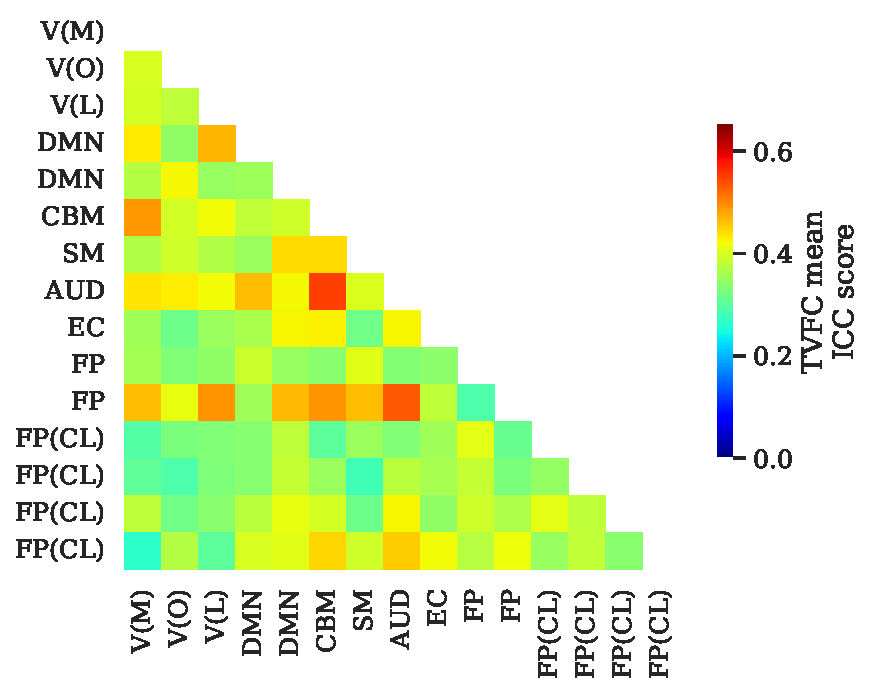
\includegraphics[width=0.28\textwidth]{fig/hcp/d15/test_retest/ICCs/correlation_mean_ICCs_DCC_joint}}
  \subcaptionbox{SW-CV\label{fig:test-retest-mean-SW-ICCs}}{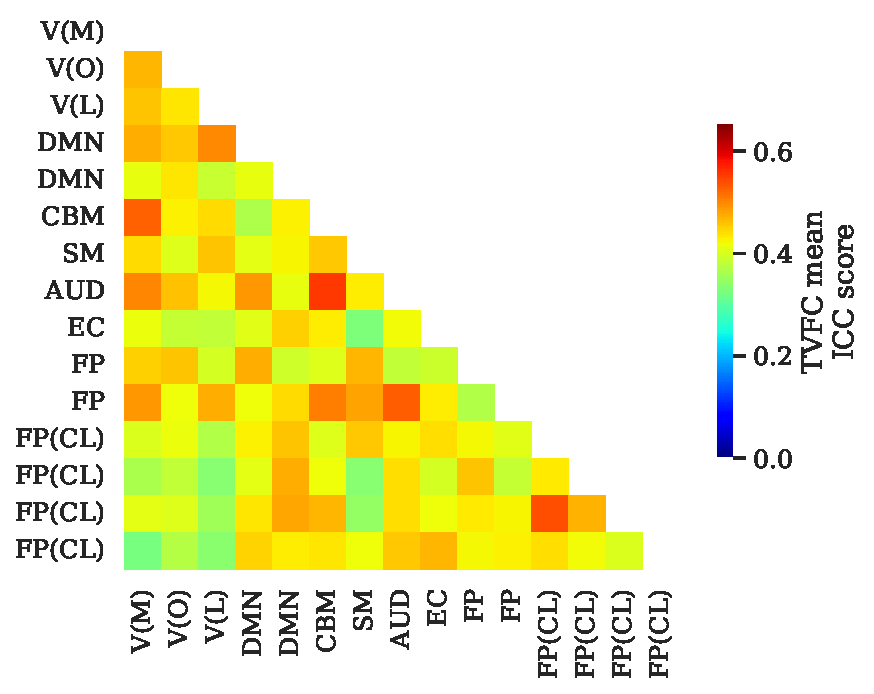
\includegraphics[width=0.28\textwidth]{fig/hcp/d15/test_retest/ICCs/correlation_mean_ICCs_SW_cross_validated}}
  \subcaptionbox{SVWP-J\label{fig:test-retest-variance-SVWP-ICCs}}{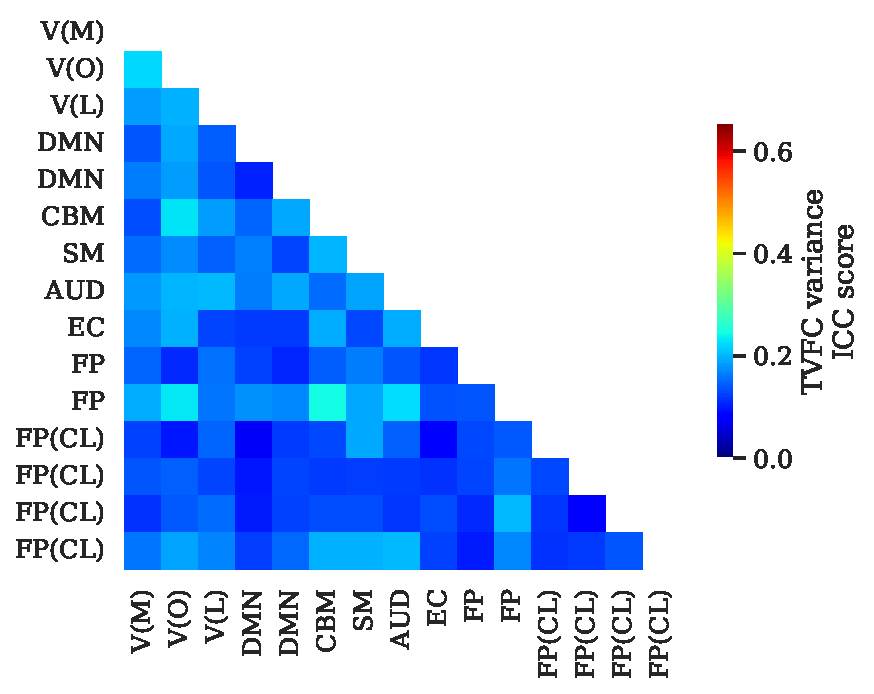
\includegraphics[width=0.28\textwidth]{fig/hcp/d15/test_retest/ICCs/correlation_variance_ICCs_SVWP_joint}}
  \subcaptionbox{DCC-J\label{fig:test-retest-variance-DCC-ICCs}}{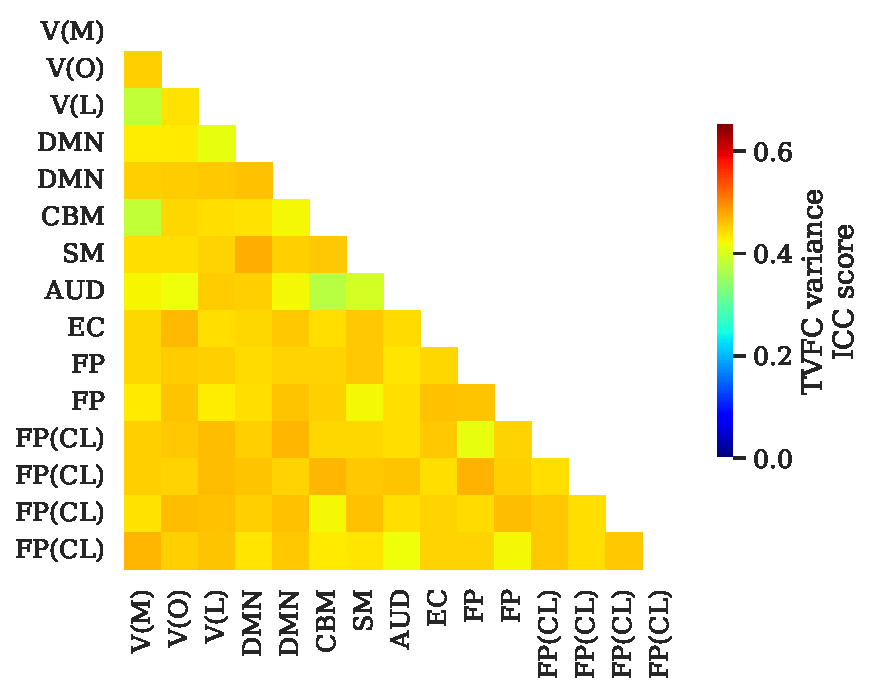
\includegraphics[width=0.28\textwidth]{fig/hcp/d15/test_retest/ICCs/correlation_variance_ICCs_DCC_joint}}
  \subcaptionbox{SW-CV\label{fig:test-retest-variance-SW-ICCs}}{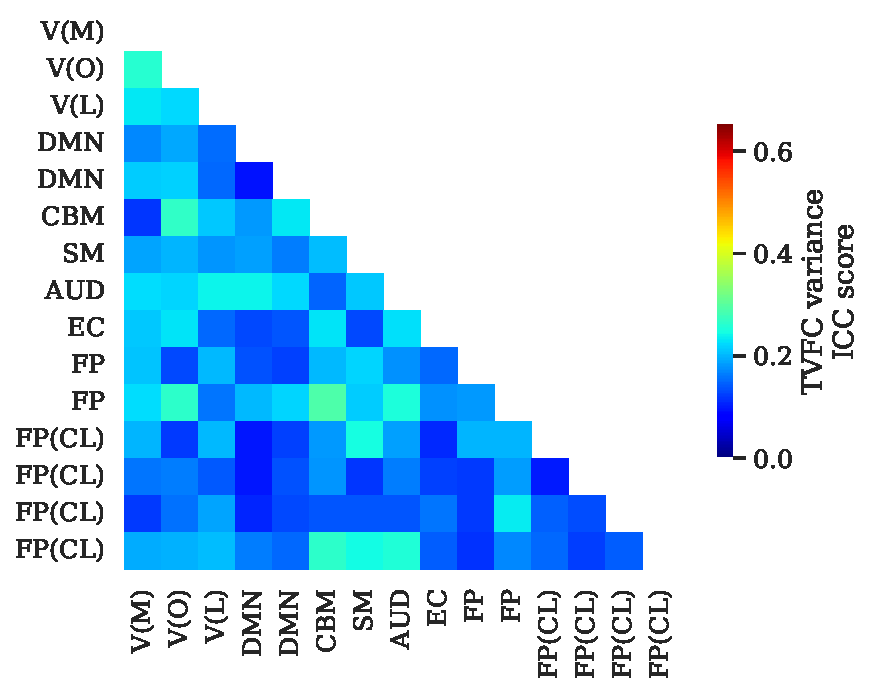
\includegraphics[width=0.28\textwidth]{fig/hcp/d15/test_retest/ICCs/correlation_variance_ICCs_SW_cross_validated}}
  \subcaptionbox{SVWP-J\label{fig:test-retest-roc-WP-ICCs}}{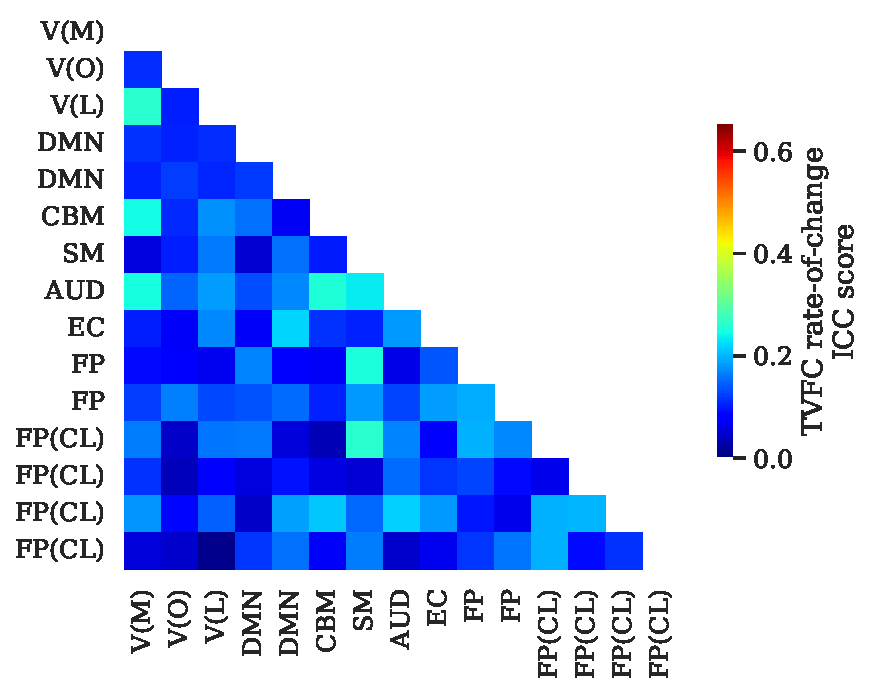
\includegraphics[width=0.28\textwidth]{fig/hcp/d15/test_retest/ICCs/correlation_rate_of_change_ICCs_SVWP_joint}}
  \subcaptionbox{DCC-J\label{fig:test-retest-roc-DCC-ICCs}}{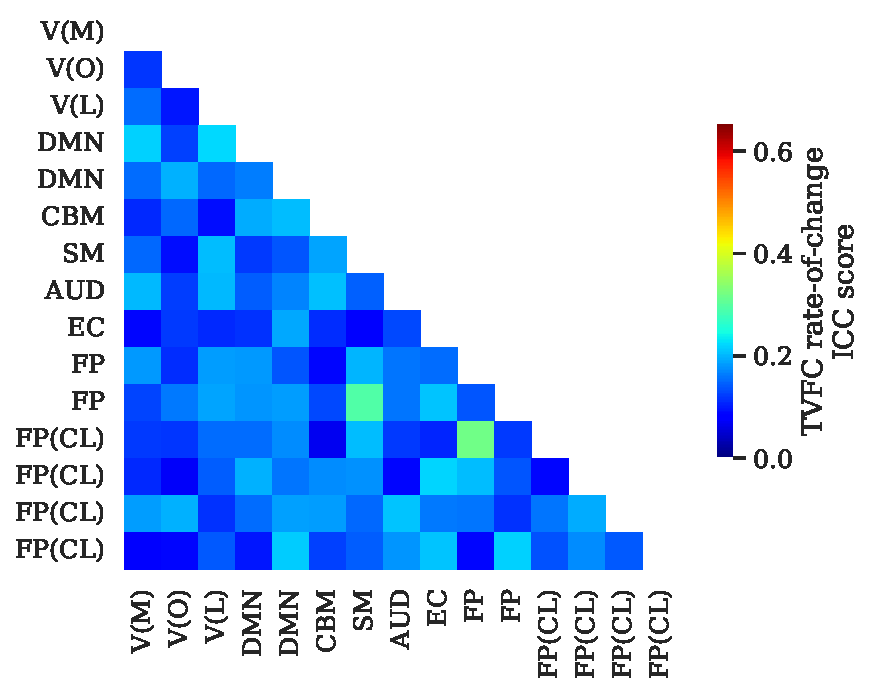
\includegraphics[width=0.28\textwidth]{fig/hcp/d15/test_retest/ICCs/correlation_rate_of_change_ICCs_DCC_joint}}
  \subcaptionbox{SW-CV\label{fig:test-retest-roc-SW-ICCs}}{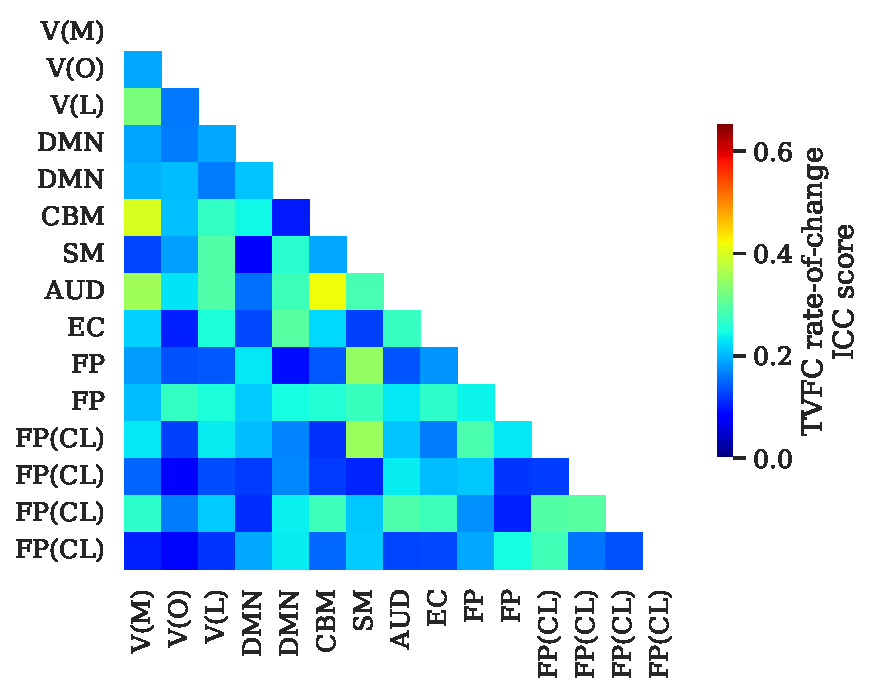
\includegraphics[width=0.28\textwidth]{fig/hcp/d15/test_retest/ICCs/correlation_rate_of_change_ICCs_SW_cross_validated}}
  \caption{
    HCP benchmark test-retest robustness edgewise ICC(2,1) scores across four scans of estimated TVFC on $D = 15$ ICA-based data.
    Reliability of TVFC means (top), variance (middle), and rate-of-change (bottom row) are shown.
    For interpretation, ICA components are mapped to FNs.
    Visual (V): medial (M), occipital (O), lateral (L); Default Mode Network (DMN); Cerebellum (CBM); Sensorimotor (SM); Auditory (AUD); Executive Control (EC); Frontoparietal (FP) with Cognition-Language (CL) subset.
  }\label{fig:hcp-results-test-retest-ICCs-d15}
\end{figure}


\info[inline]{Paragraph: Discuss additional subject measures.}
Morphometricity scores for additional subject measures (including social-emotional and other measures) can be found in \cref{appendix:hcp-more-results}.
The variance explained for these measures is generally much lower.
This shows that \gls{fc} may capture cognitive individual differences better than affective ones.
Comparing to prior findings, we replicate \textcite{Dubois2018} and find that the Big Five personality trait of `openness to experience' is best explained by \gls{sfc}~\parencite[see also][]{Beaty2018}.

This morphometricity analysis is based on a linear model.
To understand more complex dynamics captured by the various methods, we may need to run models such as \glspl{rnn}.
If we are solely interested in making subject measure predictions, we could also bypass covariance structure estimation entirely.
However, we reiterate that our goal here is not to build the best model for subject measure prediction, but to benchmark \gls{tvfc} estimation methods.

%%
\subsubsection{Test-retest robustness benchmark}
%%

The \gls{icc} scores per edge are shown in \cref{fig:hcp-results-test-retest-ICCs-d15}, analogous to figures 4B and 4C in \textcite{Choe2017}.
Each \gls{ica} component is labeled with one of the 10 BrainMap components from \textcite{Smith2009} with most overlap (see \cref{fig:brainmap-functional-networks}).
%
Some edges are shown to be more robust than others, consistently across methods (see e.g.~CBM-AUD).
However, this increased robustness does not generalize across summary measures.
Furthermore, \gls{dcc} mean \gls{tvfc} edges are slightly less robust than the other methods, but its variance is much more robust.
This outperformance over \gls{sw} methods was found by \textcite{Choe2017} too.
Overall, robustness of connectivity strengths is much higher than for the dynamic summary measures.

The omnibus (whole brain) I2C2 scores for the reliability of the \gls{tvfc} mean, variance, and rate-of-change are shown in \cref{fig:hcp-results-test-retest-I2C2-scores-d15}.
Just like \textcite{Choe2017}, we do not find much disagreement between \gls{icc} and I2C2 scores.
The I2C2 score is a good representation of the ``average'' \gls{icc} score over all edges from \cref{fig:hcp-results-test-retest-ICCs-d15}.
We posit that using I2C2 scores is a good measure for whole-brain test-retest robustness.
However, in some cases we may be interested in the robustness of particular edges.
For comparison, \textcite{Choe2017} found respective values for the \gls{tvfc} mean between 0.44 and 0.48 for all methods.
We find similar values for all our methods.
They found respective values for the \gls{tvfc} variance between 0.16 and 0.30 for \gls{sw} methods (with different window lengths) and 0.49 for \gls{dcc}.
That is, they also found more variety between methods in I2C2 values for \gls{tvfc} variances than for \gls{tvfc} means.


\begin{figure}[t]
  \centering
  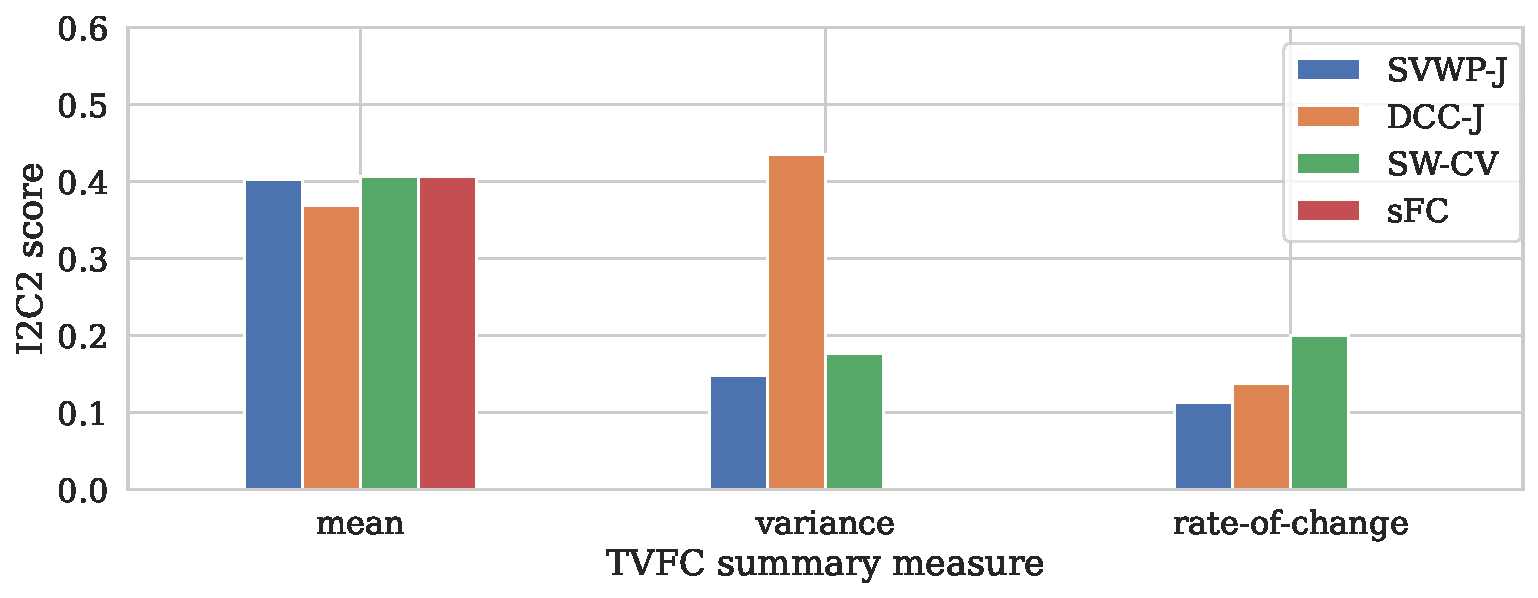
\includegraphics[width=\textwidth]{fig/hcp/d15/test_retest/I2C2/correlation_I2C2_scores}
  \caption{
    HCP benchmark test-retest robustness I2C2 omnibus scores for mean, variance, and rate-of-change TVFC summary measures.
  }\label{fig:hcp-results-test-retest-I2C2-scores-d15}
\end{figure}


Following up from \cref{subsec:model-features}, we can also compute the \gls{icc} score for the learned \gls{svwp} kernel parameters.
We find a score of 0.29 for the kernel variance and 0.48 for the kernel lengthscales $l$.
Taking the categories from \textcite{Cicchetti1994}, these can be considered `poor' and `fair', respectively.
These are high in comparison to the scores for the summary measures.
%
How should we interpret these results?
From the perspective of viewing this as a prediction problem, we can view this test-retest problem as the following question: ``Given the first scan, how well can we predict which scan is that subject's subsequent scan?''.
The issue here is not just to look at test-retest scores, but to use them to justify using one method over another.
In that light, we just expect a method to generate \emph{any} feature that may help us do this.
The method with the best score from any such feature can be considered stronger.
%
Furthermore, it is not clear how having more robust estimations across scans is related to actual performance on subsequent tasks.
We will discuss this point more in \cref{subsec:benchmarking-discussion-rs-fmri}.

%%
\subsubsection{Imputation benchmark}
%%

Results for the imputation study are shown in \cref{fig:hcp-results-LEOO-multivariate}.
Shown are results under the \gls{leoo} train and test set creation.
The \gls{wp} and \gls{sw-cv} methods outperform the other methods.
The poor performance of \gls{dcc} here may be due to not learning the correct mean.


\begin{figure}[t]
  \centering
  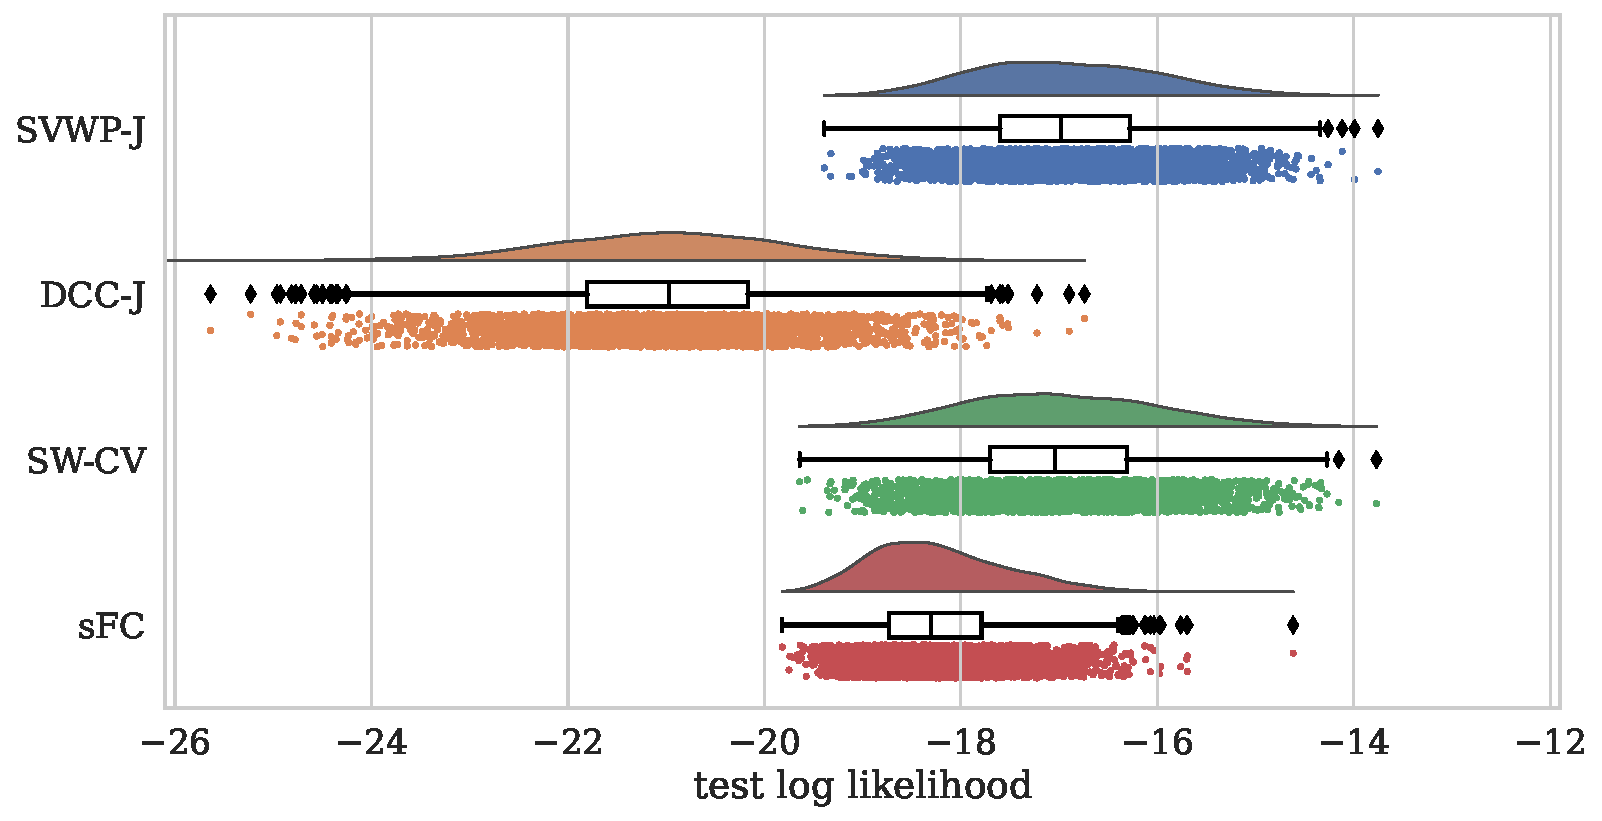
\includegraphics[width=\textwidth]{fig/hcp/d15/imputation_study/LEOO_multivariate_test_log_likelihoods_raincloud}
  \caption{
    HCP benchmark imputation results under LEOO train-test split.
    The boxplot shows median, quartiles, and outliers.
  }\label{fig:hcp-results-LEOO-multivariate}
\end{figure}


\begin{figure}[t]
  \centering
  \subcaptionbox{SVWP-J\label{fig:edgewise-imputation-benchmark-SVWP}}{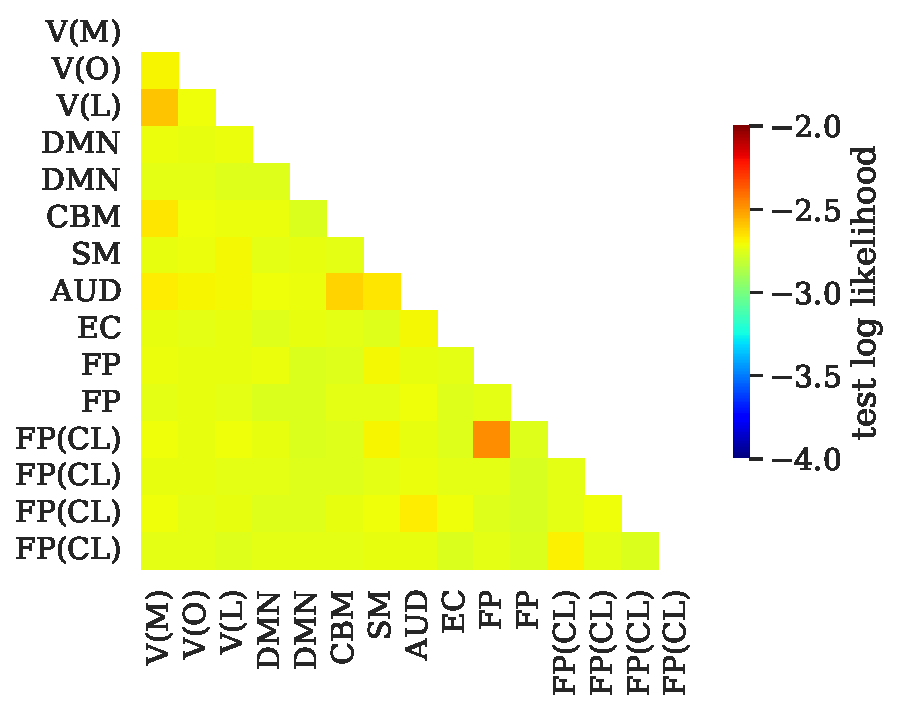
\includegraphics[width=0.45\textwidth]{fig/hcp/d15/imputation_study/LEOO_multivariate_test_log_likelihoods_edgewise_SVWP_joint}}
  \subcaptionbox{DCC-J\label{fig:edgewise-imputation-benchmark-DCC}}{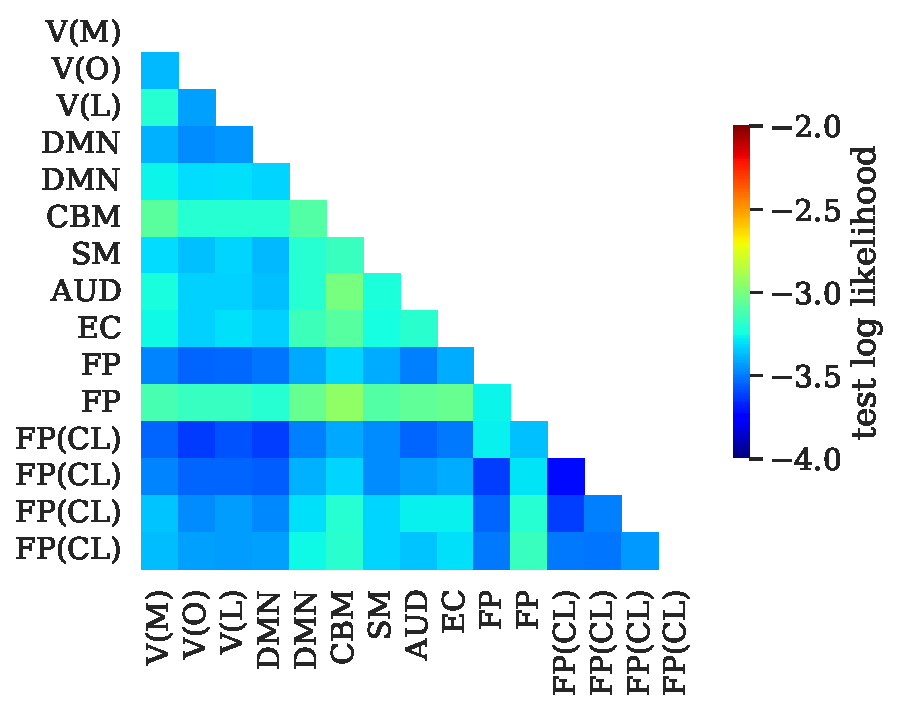
\includegraphics[width=0.45\textwidth]{fig/hcp/d15/imputation_study/LEOO_multivariate_test_log_likelihoods_edgewise_DCC_joint}}
  \subcaptionbox{SW-CV\label{fig:edgewise-imputation-benchmark-SW-CV}}{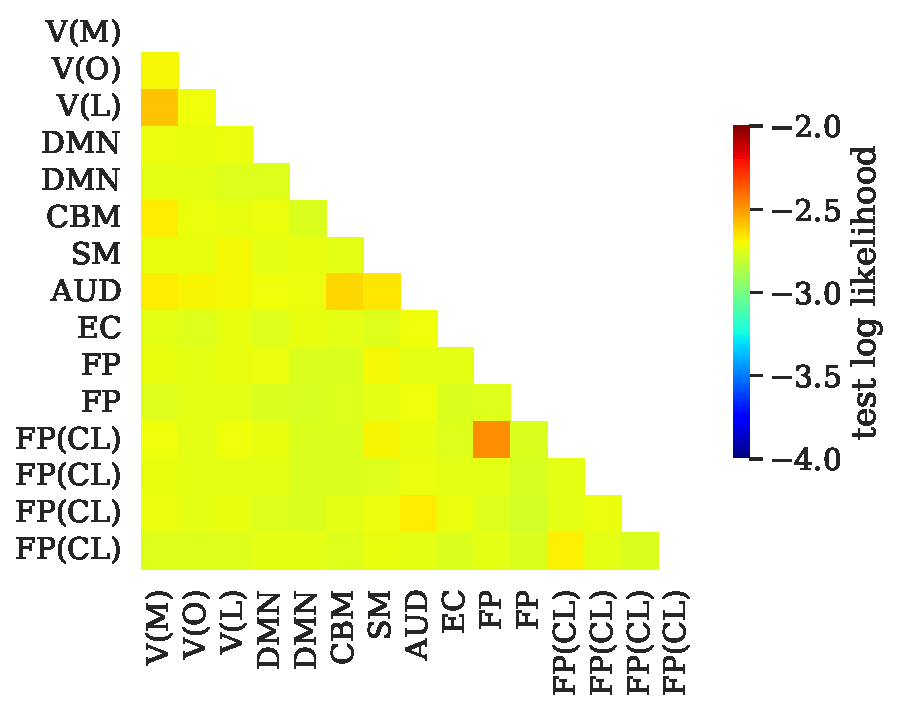
\includegraphics[width=0.45\textwidth]{fig/hcp/d15/imputation_study/LEOO_multivariate_test_log_likelihoods_edgewise_SW_cross_validated}}
  \subcaptionbox{sFC\label{fig:edgewise-imputation-benchmark-STATIC}}{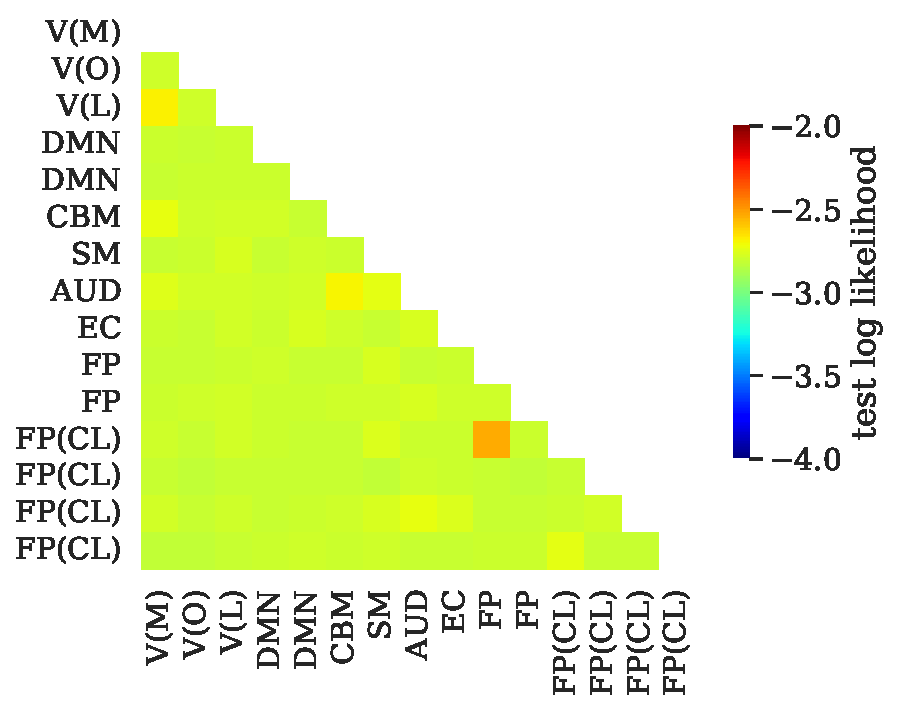
\includegraphics[width=0.45\textwidth]{fig/hcp/d15/imputation_study/LEOO_multivariate_test_log_likelihoods_edgewise_sFC}}
  \caption{
    HCP benchmark edgewise imputation results for various methods on $D = 15$ ICA-based data.
    The equivalent of mean test log likelihoods from \cref{fig:hcp-results-LEOO-multivariate} are shown for each edge individually.
    For interpretation, ICA components are mapped to FNs.
    Visual (V): medial (M), occipital (O), lateral (L); Default Mode Network (DMN); Cerebellum (CBM); Sensorimotor (SM); Auditory (AUD); Executive Control (EC); Frontoparietal (FP) with Cognition-Language (CL) subset.
  }\label{fig:hcp-results-edgewise-imputation-benchmark}
\end{figure}


This is a whole-brain analysis.
However, there may be certain edges where \gls{svwp} performance is similar to the static approach (i.e.~static edges) and some where it outperforms (i.e.~dynamic edges).
In fact, we posit that outperformance over static estimates can be considered a proxy for a statistical test of whether there is any time-varying structure~\parencite[see also][]{Zalesky2014, Hindriks2016}.
This point was made earlier based on \cref{fig:sim-imputation-study-d2-null,fig:sim-imputation-study-d2-periodic-1}.
To further explore this proposal, the population-level edgewise imputation benchmark scores (averaged over all subjects) are plotted in \cref{fig:hcp-results-edgewise-imputation-benchmark}.
First, caution is advised when interpreting these.
Certain edges have high performance on this imputation benchmark, see e.g.~FP-FP(CL), but this may simply be due to this edge being very static (and thus easier to fit).
Comparison between edges is less insightful than comparison for the same edge \emph{between} estimation methods.
%
We find \gls{svwp} outperformance over \gls{sfc} is stronger in certain edges.
This may point to these edges changing more across time.
And indeed, these edges have higher variance and rate-of-change summary measures (see \cref{fig:HCP-model-estimates-summary-measures-var-SVWP,fig:HCP-model-estimates-summary-measures-roc-SVWP}).

%%
\subsubsection{Brain state analysis}
%%

Extracted brain states for \gls{svwp}, \gls{dcc}, and \gls{sw-cv} are shown in \cref{fig:hcp-results-brain-states-svwp,fig:hcp-results-brain-states-dcc,fig:hcp-results-brain-states-sw-cv}, respectively.
Interestingly, the extracted brain states for \gls{svwp} and \gls{sw-cv} estimates look similar.
The first brain state also looks like the \gls{sfc} estimates, as expected~\parencite{Allen2014}.

Apart from the extracted brain states, we are also interested in the dynamics and transitions of brain states.
The number of brain state change points per method per subject is shown in \cref{fig:hcp-brain-state-change-point-counts}.
Our intuition from \cref{fig:hcp-model-estimates-example} is confirmed; \gls{sw-cv} predicts many more brain state switches than \gls{svwp} (even though the state centroids are similar).
Furthermore, we see that the spread across subjects is large for \gls{dcc}, with many subjects having no change points and others a great many.


\begin{figure}[t]
  \centering
  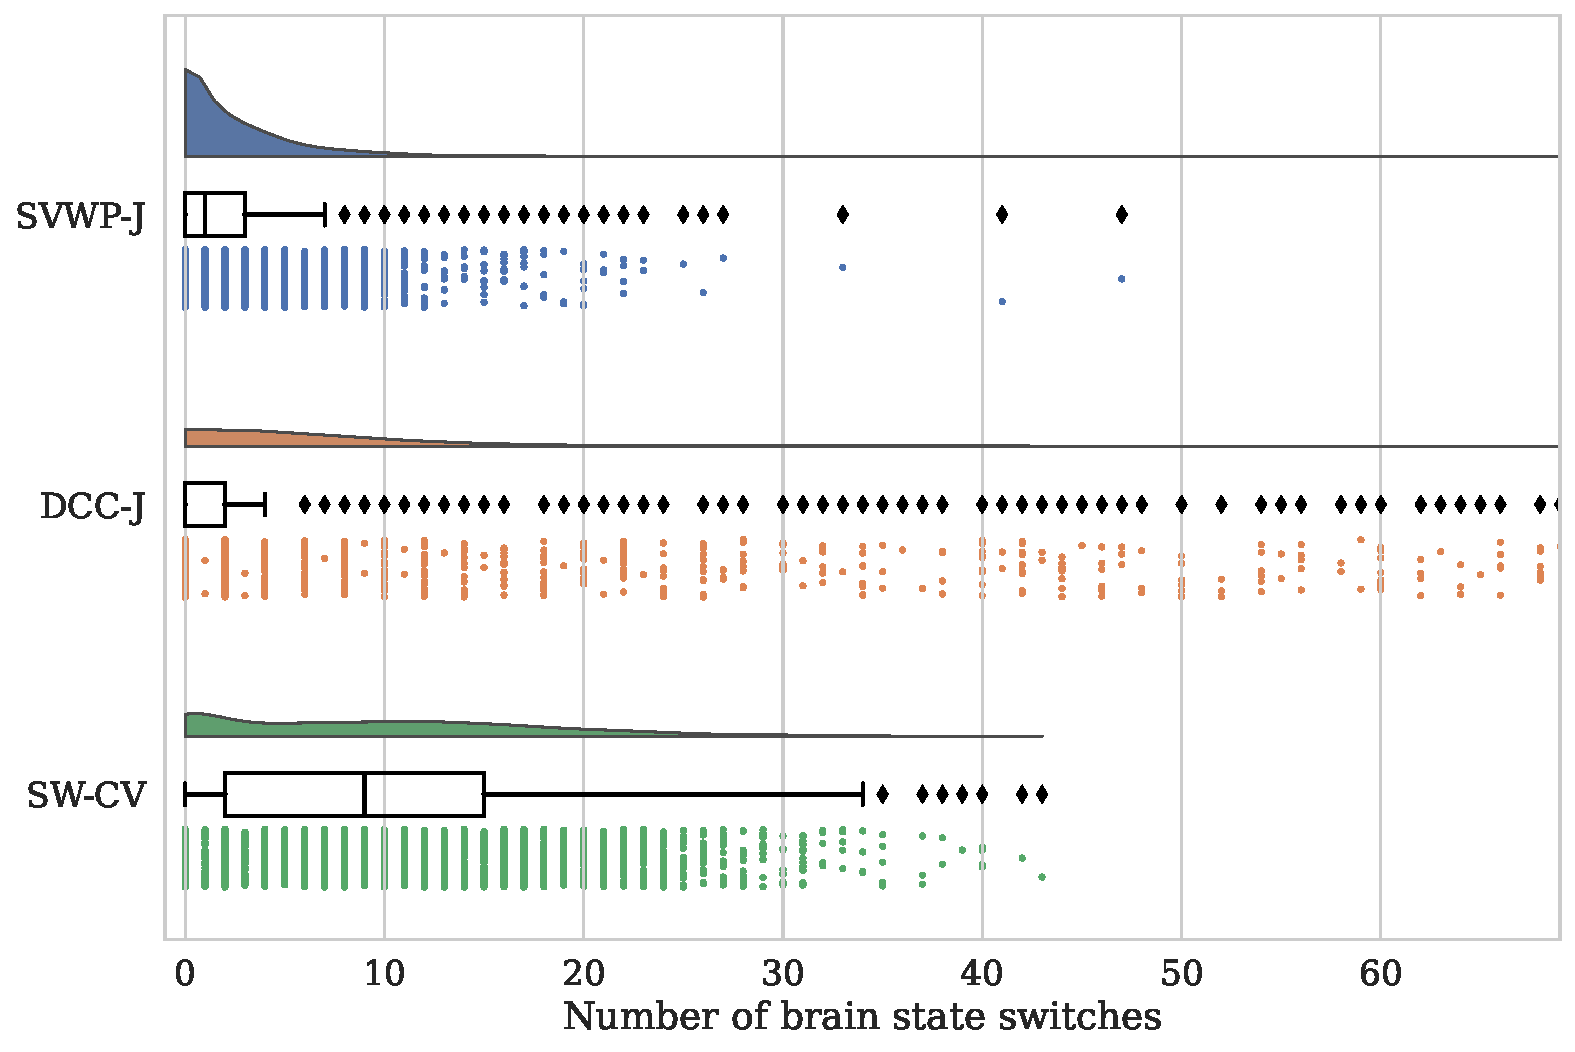
\includegraphics[width=\textwidth]{fig/hcp/d15/brain_states/k03/brain_state_switch_count}
  \caption{
    HCP brain state analysis number of brain state change points per TVFC estimation method.
    Total number of time points is $N = 1200$.
    Run on multivariate (all $D = 15$ time series) HCP data.
    The boxplot shows median, quartiles, and outliers.
  }\label{fig:hcp-brain-state-change-point-counts}
\end{figure}


%%
\subsection{Task-based fMRI}\label{subsec:rockland-results}
%%

First, we compare the \gls{vwp} kernel lengthscales to the optimal learned window length again, shown in \cref{fig:rockland-relationship-lengthscale-optimal-window-length}.
We do not find a relationship between the two.
This may indicate a failure of one (or both) of these methods to capture anything meaningful, or the approaches to focus on distinct aspects of the data.
Alternatively, these hyperparameters may in fact not be crucial to the estimates, these being driven much more by the actual observations.


\begin{figure}[t]
  \centering
  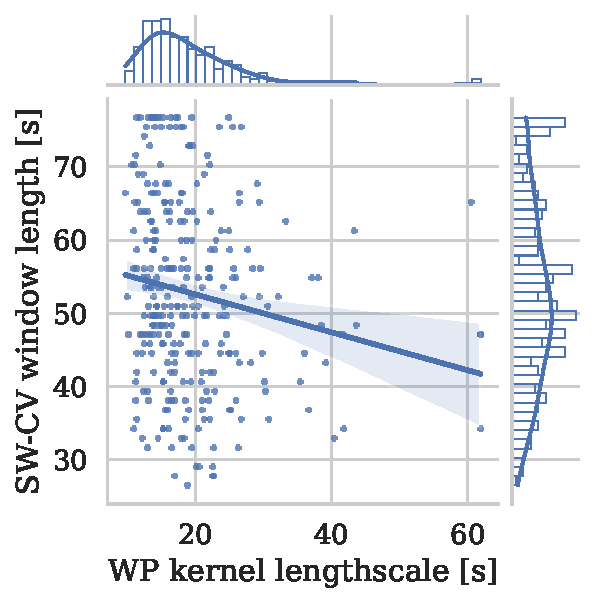
\includegraphics[width=0.45\textwidth]{fig/rockland/CHECKERBOARD645/lengthscale_optimal_window_length_relations}
  \caption{
    Rockland benchmark relationship between learned VWP kernel lengthscales (scaled to time series length) and SW-CV optimal window length.
    Each dot represents one of 286 Rockland subjects.
    Full time series is 154.8 seconds long.
  }\label{fig:rockland-relationship-lengthscale-optimal-window-length}
\end{figure}


We start with a visual inspection of model \gls{tvfc} estimates, shown in \cref{fig:rockland-results-tvfc-predictions}.
Just like the node time series plot, since we have an external task, we can average estimates across all subjects.


\begin{figure}[ht]
  \centering
  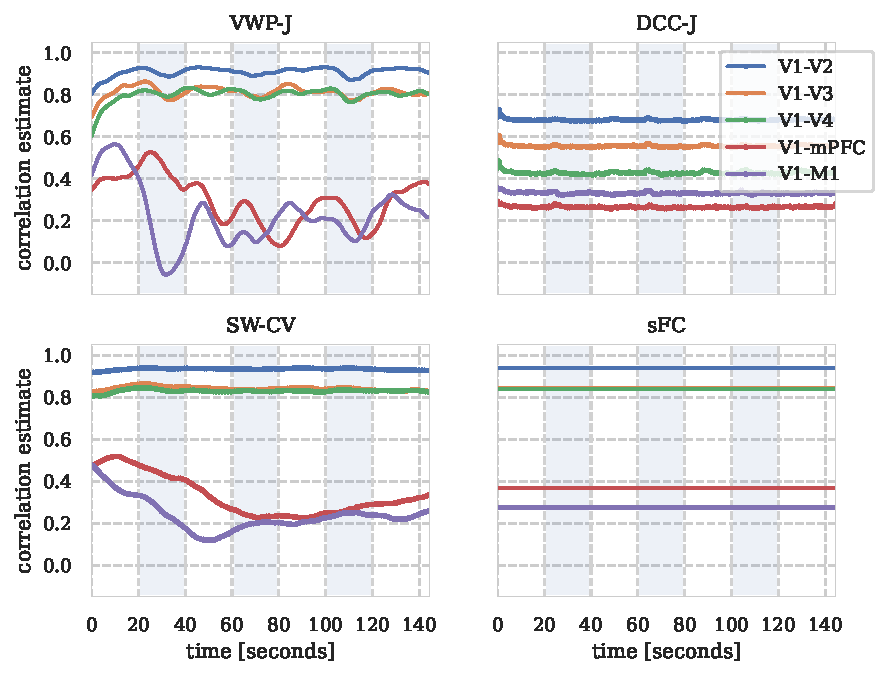
\includegraphics[width=\textwidth]{fig/rockland/CHECKERBOARD645/TVFC_predictions/all_subjects_joint_correlations}
  \caption{
    Rockland benchmark model TVFC estimates.
    Shaded areas indicate presence of external visual stimulus.
    Average estimates over all 286 subjects.
  }\label{fig:rockland-results-tvfc-predictions}
\end{figure}


As discussed, we expect that correlation between \gls{v1} and other regions should decrease as we move up and away from the visual cortex hierarchy.
We do in fact observe this from all models: connectivity with V2 is highest, followed by V3, V4, \gls{mpfc}, and connectivity strength with \gls{m1} is lowest.
However, the mean \gls{tvfc} is quite different across estimation methods, and often quite different from the \gls{sfc} estimate.
This also highlights how important the choice of \gls{tvfc} estimation method can be.

%%
\subsubsection{External stimuli prediction}
%%

Extracted $\textbf{\beta}$ parameters from our \gls{glm} are shown in \cref{fig:rockland-results-glm-betas}.
%
As expected, the \gls{sfc} cannot capture any time-varying structure.
Therefore, all drift parameters, as well as weights for task-related regressors are set to zero.
Instead, the full \gls{sfc} estimates are captured by the constant (offset) parameter of the design matrix.
%
In terms of other models, we see the \gls{vwp} model having the largest estimated task-related $\textbf{\beta}$ parameters.
Interestingly, the within-visual cortex edges have the most predictive power.
As expected from the visual inspection, the \gls{glm} has removed negative trends for \gls{v1}--\gls{mpfc} and \gls{v1}--\gls{m1}.
We conclude that the \gls{vwp} estimates have captured the most of the external task.


\begin{figure}[ht]
  \centering
  \subcaptionbox{VWP-J\label{fig:rockland-results-glm-betas-VWP}}{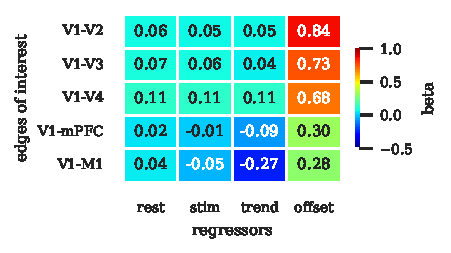
\includegraphics[width=0.48\textwidth]{fig/rockland/CHECKERBOARD645/prediction_benchmark/GLM_beta_VWP_joint}}
  \subcaptionbox{DCC-J\label{fig:rockland-results-glm-betas-DCC}}{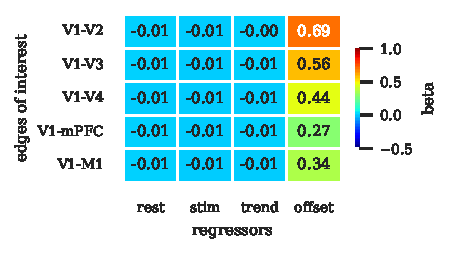
\includegraphics[width=0.48\textwidth]{fig/rockland/CHECKERBOARD645/prediction_benchmark/GLM_beta_DCC_joint}}
  \subcaptionbox{SW-CV\label{fig:rockland-results-glm-betas-SW-CV}}{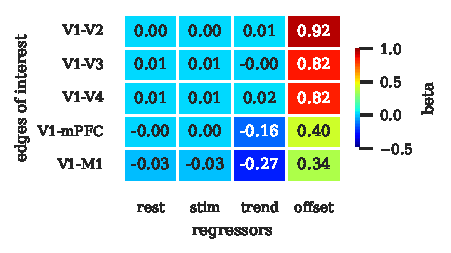
\includegraphics[width=0.48\textwidth]{fig/rockland/CHECKERBOARD645/prediction_benchmark/GLM_beta_SW_cross_validated}}
  \subcaptionbox{sFC\label{fig:rockland-results-glm-betas-sFC}}{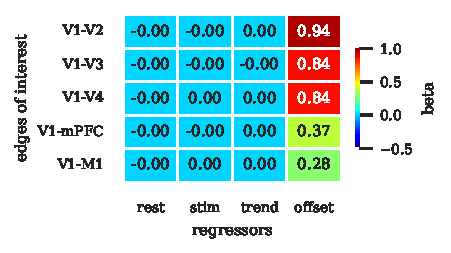
\includegraphics[width=0.48\textwidth]{fig/rockland/CHECKERBOARD645/prediction_benchmark/GLM_beta_sFC}}
  \caption{
    Rockland benchmark GLM $\beta$ (beta) parameters per TVFC estimation method.
    Values indicate learned weights.
    Higher values indicate that the GLM uses the respective design matrix features more.
    The VWP TVFC estimates are most useful for predicting the presence of the external stimulus (rest and stim columns).
  }\label{fig:rockland-results-glm-betas}
\end{figure}


%%
\subsubsection{Imputation benchmark}
%%

The imputation benchmark results (\cref{fig:rockland-results-imputation-benchmark}) show strong performance for the \gls{vwp} model and weak performance for \gls{dcc}.
\gls{sw-cv} estimate likelihoods are similar to \gls{sfc} estimates.
This may have been expected based on the visual inspection of model estimates; the \gls{sw-cv} approach found the right mean but failed to capture the dynamics.
%
As such, we show strong correspondence of performance on the imputation benchmark with the external task prediction benchmark.


\begin{figure}[ht]
  \centering
  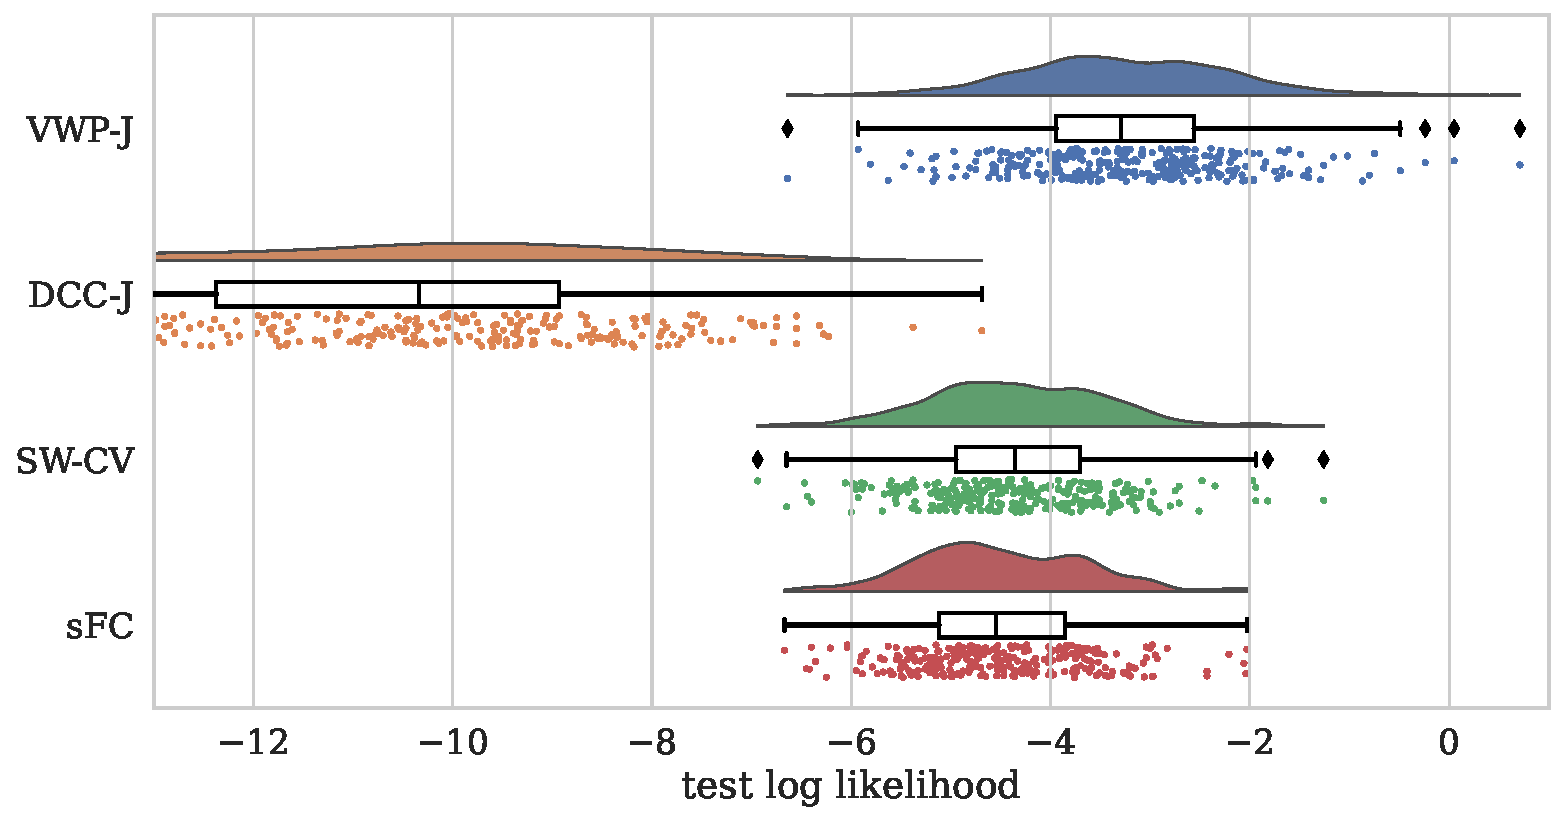
\includegraphics[width=\textwidth]{fig/rockland/CHECKERBOARD645/imputation_study/LEOO_test_log_likelihoods_raincloud}
  \caption{
    Rockland benchmark imputation results under LEOO train-test split.
    Run on~286~Rockland data subjects.
    The boxplot shows median, quartiles, and outliers.
  }\label{fig:rockland-results-imputation-benchmark}
\end{figure}
